\documentclass{article}
\usepackage[utf8]{inputenc}
\usepackage{geometry}
\geometry{
	a4paper,
	total={170mm,257mm},
	left=20mm,
	top=20mm,
}
\usepackage{graphicx}
\usepackage[dvipsnames]{xcolor}
\graphicspath{{images/}}
\usepackage{svg}
\usepackage{titling}
\usepackage[american,RPvoltages]{circuiTikz}
\usepackage{tikz, tikz-cd}
\usepackage{pgfplots}
\usepackage{siunitx}
\usepackage{float}
\usepackage{enumitem}
\usepackage{amsmath,amsfonts,stmaryrd,amssymb} % Math packages
\usepackage{tcolorbox}
\usepackage{pdfpages}
\title{El Temporizador 555}
%\author{Rodrigo Castillejos}
\author{Rodrigo}
\date{Enero 2025}


\usepackage{fancyhdr}
\fancypagestyle{plain}{%  the preset of fancyhdr 
	\fancyhf{} % clear all header and footer fields
	\fancyfoot[L]{\thedate}
	\fancyhead[L]{Temporizador 555}
	\fancyhead[R]{\theauthor}
}
\makeatletter
\def\@maketitle{%
	\newpage
	\null
	\vskip 1em%
	\begin{center}%
		\let \footnote \thanks
		{\LARGE \@title \par}%
		\vskip 1em%
		%{\large \@date}%
	\end{center}%
	\par
	\vskip 1em}
\makeatother

\renewcommand{\figurename}{Figura}
%\usepackage[color=ForestGreen!15,angle=45]{draftwatermark}
%\SetWatermarkText{CONFIDENTIAL\\COPY FOR\\ POCA POCA}
%\SetWatermarkScale{2.5}

\usepackage{lipsum}  
%\usepackage{cmbright}
%\usepackage{mathpazo}
%\usepackage{ccfonts,eulervm}
 \usepackage[T1]{fontenc}
 \usepackage{ccfonts}
%\usepackage[math]{anttor}
%\usepackage{antpolt}
 %\usepackage{fouriernc}
%\usepackage[utopia]{mathdesign}
%---------------------------------------------------
\tikzset{flipflop myRS/.style={flipflop,
		 flipflop def={t1=R, t3=S, t6=Q, t4={\ctikztextnot{Q}}, tu={\ctikztextnot{RST}}, nu=1, n4=1 }}
	}
	
\tikzset{flipflop myFFRS/.style={flipflop,
		flipflop def={t1=R, t3=S, t6=Q, t4={\ctikztextnot{Q}}, n4=1 }}
}
%---------------------------------------------------
\setlength\parindent{0pt}


\begin{document}
	
\maketitle
	
\noindent\begin{tabular}{@{}ll}
Author & \theauthor\\
\end{tabular}
	
\section*{Introducción}
El temporizador 555 es un dispositivo versátil y muy utilizado, porque puede ser configurado de dos modos distintos, bien como multivibrador monoestable o como multivibrador astable (oscilador). Un multivibrador astable no tiene estados estables y varía (oscila), por tanto, una y otra vez entre dos estados inestables, sin utilizar un circuito de disparo externo.

\section*{Diagrama de bloques funcional}
\begin{figure}[H]
	\centering	
	\begin{tikzpicture}[scale=0.8]
		\ctikzset{bipoles/thickness=4}
		\ctikzset{monopoles/vcc/arrow={Stealth[width=6pt,length=9pt]}}
		\ctikzset{monopoles/vee/arrow={Stealth[width=6pt,length=9pt]}}
		\node[flipflop myRS] (RS) at (0,0){};
		\draw (RS.pin 1) to [short] ++(-1,0) -- ++(0,1) -- ++(-1,0) coordinate (p1);
		\draw (p1) node[op amp, noinv input up, anchor=out](OA1){$CM_1$};
		\draw (RS.pin 3) to[short] ++(-1,0) -- ++(0,-1) -- ++(-1,0) coordinate (p2);
		\draw (p2) node[op amp, noinv input up, anchor=out](OA2){$CM_2$};
		\draw (OA1.-) to[short] ++(-1,0) coordinate (p3);
		\draw (OA2.+) to[short] ++(-1,0) coordinate (p4);
		\draw (p3) to[R, *-*, l=$R$] (p4);
		\draw (RS.pin 4) to[short] ++(2,0) to[short] ++(0,7) to[short] ++(-5,0)
		      to[R] ++(-3,0) coordinate(p5);
		\draw (p5) node[npn, anchor=B, xscale=-1](Q){}	;
		\draw (Q.E) node[ground]{};
		\draw (RS.pin 6) to[short, -o] ++(4,0) node[right]{$Out$} node[below]{$3$};
		\draw (OA2.-) to[short, -o] ++(-3,0) node[left]{$Trigger$} node[below]{$2$};
		\draw (p4) to[R, l=$R$] ++(0,-5) node[ground]{$\,GND$} node[left]{$1$} coordinate(x3);
		\draw (p3) to[short, -o] ++(-2,0) node[left]{$Voltage$} node[below left=1mm]{$control$} node[below]{$5$};
		\draw (OA1.+) to[short, -o] ++(-3,0) coordinate (p6) node[left]{$Threshold$} node[below]{$6$};
		\draw (Q.C) to[short] ++(0,0.5) coordinate (p7);
		\draw (p7) to[short, -o] (p7 -| p6);
		\draw (p3) to[R, l_=$R$] ++(0,5)
              to[short] ++(0,2) coordinate(p8) node[vcc](VCC){$+V_{CC}$} node[right]{$VCC$} node[left]{$8$};
        \draw (RS.up) coordinate(x1) to[short] (x1 |- p8) node[vcc](VCC){$+V_{CC}$} node[right]{$Reset$} node[left]{$4$} coordinate(x2);
        \draw[black, dashed, thick] (-9,8) rectangle (4.5,-6);
        \draw[<-](p3)++(-0.1,0.1) -- ++(-0.5,0.6) coordinate(a1);
        \draw (a1) node[left=-1mm]{$\frac{2V_{cc}}{3}$};
        \draw[<-](p4)++(-0.1,-0.1) -- ++(-0.5,-0.6) coordinate(a2);
        \draw (a2) node[left=-1mm]{$\frac{V_{cc}}{3}$};
        \draw (Q.B) node[left=7mm]{$Q_1$};
	\end{tikzpicture}
	\caption{Diagrama de bloques interno del integrado 555}	
	\label{fig:figura1}
\end{figure}

\newpage

\section*{Funcionamiento básico}
El diagrama de bloques del 555 se muestra en la figura 1, el \textit{timer} consiste de dos comparadores $CM_1$ y $CM_2$, un latch $RS$, un transistor de descarga $Q_1$ y una red divisora de voltaje.

\subsection*{El comparador}
Los comparadores son dispositivos cuyas salidas permanecen  a nivel $ALTO$ o $1$ lógico cuando la tensión de entrada positiva ($+$) es mayor que la tensión de entrada negativa ($-$) y permanece a un nivel $BAJO$ o $0$ lógico cuando la tensión de entrada negativa ($-$) es mayor que la tensión de entrada positiva ($+$). Matemáticamente, el voltaje de salida de un comparador está dado por:

\begin{align}
    V_o =  
	\begin{cases}
		+V_{cc} \, ( \textrm{1 lógico}), & V_1 > V_2 \\
		-V_{cc} \, (\textrm{0 lógico}), & V_1 < V_2
	\end{cases} = 
	\begin{cases}
		+V_{cc} \, (\textrm{1 lógico}), & V_1 > V_2 \\
		GND \, = \, \qty{0}{\volt} \, (\textrm{0 lógico}), & V_1 < V_2
	\end{cases}
\end{align} 

De la ecuación 1, el primer caso es cuando se alimenta al comparador con fuentes bipolares, por ejemplo $\pm \qty{15}{\volt}$, el segundo caso es cuando se usa una fuente simple, por ejemplo +\qty{5}{\volt}.

\begin{figure}[H]
	\centering
	\begin{tikzpicture}[scale=0.8]
		\ctikzset{bipoles/thickness=4}
		\ctikzset{monopoles/vcc/arrow={Stealth[width=6pt,length=9pt]}}
		\ctikzset{monopoles/vee/arrow={Stealth[width=6pt,length=9pt]}}
		\draw (0,0) node[op amp, noinv input up, anchor=out](OA1){};
		\draw (OA1.+) to[short, -o] ++(-2,0) node[left]{$V_1$};
		\draw (OA1.-) to[short, -o] ++(-2,0) node[left]{$V_2$};
		\draw (OA1.out) to[short, -o] ++(1,0) node[right]{$V_o$};
	\end{tikzpicture}
	\caption{Símbolo de un comparador}	
	\label{fig:figura2}
\end{figure}

\subsection*{Divisor de tensión}
El divisor de voltaje del circuito de la figura 1 y que se muestra nuevamente en la figura 3, está compuesto por tres resistencias, las cuales establecen el voltaje en la terminal inversora de $CM_1$ a $\frac{2V_{cc}}{3}$ y un voltaje en la terminal no inversora de $CM_2$ de $\frac{V_{cc}}{3}$

\begin{figure}[H]
	\centering	
	\begin{tikzpicture}[scale=0.8]
		\ctikzset{bipoles/thickness=4}
		\ctikzset{monopoles/vcc/arrow={Stealth[width=6pt,length=9pt]}}
		\ctikzset{monopoles/vee/arrow={Stealth[width=6pt,length=9pt]}}
		\draw (0,0) node[ground]{} to[R, l_=$R_3$] ++ (0,3) coordinate(p1)
		      to[R, l_=$R_2$] ++(0,3) coordinate(p2)
		      to[R, l_=$R_1$] ++(0,3) node[vcc](VCC){$+V_{CC}$};
		\draw (p1) to[short, *-o] ++(2,0) node[right]{$Al \, comparador$} node[below right]{$CM_2$} node[below left]{$V_{CM_2}$};
		\draw (p2) to[short, *-o] ++(2,0) node[right]{$Al \, comparador$} node[below right]{$CM_1$} node[below left]{$V_{CM_1}$};		      
	\end{tikzpicture}
	\caption{Red divisora de voltaje que establece el voltaje en los terminales de entrada de los comparadores.}	
	\label{fig:figura3}
\end{figure}

El voltaje a través de $R_3$ establece un voltaje de $\frac{V_{cc}}{3}$ en la terminal positiva del comparador $CM_2$, para comprobarlo, usamos el principio de división de voltaje obteniendo:

\begin{align}
	V_{CM_2} = \frac{R_3}{R_1 + R_2 + R_3}V_{CC}
\end{align}

Asumiendo que $R_1 =  R_2 = R_3 = R$ (como es el caso del $555$ el cual tiene tres resistores internos de igual valor), de la ecuación (2) obtenemos

\begin{align}
	V_{CM_2} = \frac{R}{3R}V_{{CC}} = \frac{1}{3}V_{CC}
\end{align}

Ahora, el voltaje a través de la terminal negativa del comparador $CM_1$ está dado por

\begin{align}
	V_{CM_1} = \frac{R_2 + R_3}{R_1 + R_2 + R_3}V_{CC}
\end{align}

De manera similar, si asumimos que las tres resistencias tienen valores idénticos, entonces:

\begin{align}
	V_{CM_1} = \frac{2R}{3R}V_{CC} = \frac{2}{3}V_{CC}
\end{align}

\subsection*{Latch SR}
Los circuitos secuenciales tienen la propiedad de que la salida depende no sólo del estado presente de su entrada, sino también de la secuencia pasada de sus entradas. En efecto, estos circuitos deben ser capaces de "recordar" la historia pasada de sus entradas con el fin de producir la salida presente. Los latches y flip-flops son dispositivos de memoria comúnmente usados en circuitos secuenciales. La principal diferencia entre un latch y un flip-flop es que lo latches no tienen entradas de reloj. Así, reservamos el término flip-flop sólo a aquellos dispositivos de memoria que cambian el estado de su salida en respuesta a una señal de reloj y no en respuesta a los datos de entrada. \\

\noindent El circuito de memoria más simple es el latch $SR$, se forma retroalimentando dos compuertas $NOR$ como se muestra en el circuito de la siguiente figura. Sus dos entradas están etiquetadas como $S$ (Set) y $R$ (Reset). Las salidas son etiquetadas como $Q$ y $\bar{Q}$, enfatizando su complementariedad. Se considera que el latch está en estado de $SET$ (es decir, almacenando un $1$ lógico) cuando $Q$ es alta y $\bar{Q}$ es bajo. Se considera que el latch está en estado de $RESET$ cuando sus estados están invertidos ($Q$ en bajo y $\bar{Q}$ en alto).

\begin{figure}[H]
	\centering	
	\begin{tikzpicture}[scale=1]
		\ctikzset{bipoles/thickness=4}
		\ctikzset{monopoles/vcc/arrow={Stealth[width=6pt,length=9pt]}}
		\ctikzset{monopoles/vee/arrow={Stealth[width=6pt,length=9pt]}}
		\draw (0,2) node[nor port] (NOR1) {}
		(1.8,2) node[anchor=east] {Q}
		(1.8,0) node[anchor=east] {$\overline{Q}$}
		(0,0) node[nor port] (NOR2) {}
		(NOR1.in 1) node[anchor=east] {R}
		(NOR2.in 2) node[anchor=east] {S}
		(NOR1.out) -- ++(0,-0.5) -- ($(NOR2.in 1) +(0,0.5)$) -- (NOR2.in 1)
		(NOR2.out) -- ++(0,+0.5) -- ($(NOR1.in 2) +(0,-0.5)$)--(NOR1.in 2);
		\draw (NOR1.out) to[short, *-o] ++(1,0);	      
		\draw (NOR2.out) to[short, *-o] ++(1,0);
		
		
		\node[flipflop myFFRS] (RS) at (5,1){};
		
		\node at (10,1) {\begin{tabular}{|cc|c|}
		$R$ & $S$ & $Q_{n+1}$ \\
		\hline %
		$0$ & $0$ & $Q_n$ \\
		$0$ & $1$ & $1$ \\
		$1$ & $0$ & $0$ \\
		$1$ & $1$ & $Not \, used$ \\
	\end{tabular}};

    \node[anchor=west] at (-1.5,-1.5){$(a) \, \textrm{circuito}$};
    \node[anchor=west] at (4,-1.5){$(b) \, \textrm{símbolo}$};
    \node[anchor=west] at (8.5,-1.5){$(c) \, \textrm{Tabla de verdad}$};
	\end{tikzpicture}
	\caption{Latch SR}	
	\label{fig:figura4}
\end{figure}

\newpage

\section{Circuito monoestable}
Un circuito monoestable es un circuito generador de pulso no redisparable. Normalmente, su salida es $0$, esto es, un nivel lógico bajo en el estado estable. Este circuito tiene sólo un estado estable. La configuración del circuito para una operación monoestable se muestra en la figura 5.

\begin{figure}[H]
	\centering	
	\begin{tikzpicture}[scale=0.8, transform shape]
		\ctikzset{muxdemux/inner label font=\small}
		\ctikzset{muxdemux/outer label font={\small\color{blue}}}
		\tikzset{ic555/.style={muxdemux,
				 muxdemux def={Lh=10, NL=6, Rh=10, NR=1, NB=2, w=6, NT=2}, %Lh = Left height, Rh = Right Heigh, w = width, NL = number of pin on the left, NR, number of pín on the right, NB = number of pins on the bottom 
				 muxdemux label={L2=Discharge, L3=Trigger, L5=Threshold, R1=Out,
					 T1={\ctikztextnot{RST}}, T2=VCC,  B1=GND, B2=Control, 
					 LU2=7, LU3=6, LU5=2, TL1=8, TL2=4, RU1=3, BL1=1, BL2=5},
				external pins width=0.4,
				draw only left pins={2,3,5},
				circuitikz/muxdemuxes/fill=blue!10}
			}
		 \node [ic555, font=\small\ttfamily,align=center](A) at (0,0) {LM555};
		 \draw (A.lpin 2) to[short] ++(-1,0) coordinate (p1);
		 \draw (A.lpin 3) to[short] ++(-1,0) coordinate (p2);
		 \draw (A.tpin 2) to[short] ++(0,1) coordinate (t2);
		 \draw (p1) to[short, *-*] (p2)
		       to[short] ++(0,-1.5) coordinate (x1);
		  \draw (p1) to[R, l=$R_1$] (p1 |- t2) coordinate (r1) to [short] (t2);
		  \draw (A.tpin 1) to[short, -*] ++(0,1) to[short] ++(0,0.2) node[vcc](VCC){$+V_{CC}$};
		  \draw (A.bpin 2) to[cC, l=$C_2$] ++(0,-1) coordinate (b2);
		  \draw (x1) to [cC, l_=$C_1$, v^=$V_c(t)$] (x1 |- b2) coordinate (c2)
		        to [short] (b2);
		  \draw (A.bpin 1) to[short, -*] ++(0,-1) node[ground]{};
		  \draw (A.lpin 5) to[short, -*] ++(-3,0) coordinate (x2);
		  \draw (x2) to[R, l=$R_2$] (x2 |- r1) to[short, -*] (r1);
		  \draw (x2) to[push button, l_=$SW_1$] (x2 |- c2) to[short, -*] (c2); 
		  \draw (x2)++(-1,0) to[short] ++(0.2,0) coordinate (arr1) to[short] ++(0,-0.7) to[short] ++(0.4,0) to[short] ++(0,0.7) to[short] ++(0.2,0);
		  \draw (x2) node[left=8mm, above=5mm]{$Trigger$};
		  \draw (x2) node[left=8mm, above=2mm]{$Input$};
		  \draw[-Stealth] (arr1) -- ++(0,-0.5);
		  \draw (A.rpin 1) to[short, -o] ++(1,0);
		  
		  \pgfplotsset{width=9cm,height=5cm,compat=1.18}
		  \begin{axis}[xshift=6cm,
		  	yshift=2cm,
		  	clip=false,
		  	axis y line=left,
		  	axis x line=middle,
		  	xlabel=$t$,
		  	ylabel=$v_I$, 
		  	axis y line= center,
		  	xmin=0,xmax=5,
		  	ymin=0,ymax=1.5,
		  	xtick={0},
		  	ytick={1},
		  	xticklabels={$$},
		  	yticklabels={$V_{CC}$},
		  	]
		  	\addplot+[line width=1pt,mark=none,const plot]
		  	coordinates {(0,1) (0.5,1) (0.5,0) (1,0) (1,1) (2,1) (2,0) (2.5,0) (2.5,1) (3.5,1) (3.5,0) (4,0) (4,1) (4.5,1)};
		  	\addplot[color = black, dashed, thick] coordinates {(0.5,0) (0.5,-1)}; %vertical1
		  	\addplot[color = black, dashed, thick] coordinates {(2,0) (2,-1)}; %vertical2
		  	\draw[Stealth-] (0.5,-0.5) node[right=8.5mm]{$T$}-- (1,-0.5);
		  	\draw[-Stealth] (1.5,-0.5) -- (2,-0.5);
		  \end{axis}
		  
		  \pgfplotsset{width=9cm,compat=1.18}
		  \begin{axis}[xshift=6cm,
		  	yshift=-2cm,
		  	clip=false,
		  	axis y line=left,
		  	axis x line=middle,
		  	xlabel=$v_I$,
		  	ylabel=$v_O$, 
		  	axis y line= center,
		  	xmin=0,xmax=5,
		  	ymin=0,ymax=1.5,
		  	xtick={0},
		  	xticklabels={$$},
		  	ytick={-1,1},
		  	yticklabels={$V_{EE}$,$V_{CC}$},
		  	]
		  	\addplot+[line width=1pt,mark=none,const plot]
		  	coordinates {(0,0) (0.5,0) (0.5,1) (1.25,1) (1.25,0) (2,0) (2,1) (2.75,1) (2.75,0) (3.5,0) (3.5,1) (4.25,1) (4.25,0)};
		  	\addplot[color = black, dashed, thick] coordinates {(0.5,0) (0.5,-1.75)}; %vertical1
		  	\addplot[color = black, dashed, thick] coordinates {(1.25,0) (1.25,-1.75)}; %vertical1
		  	\addplot[color = black, dashed, thick] coordinates {(2,0) (2,-1.75)}; %vertical1
		  	\addplot[color = black, dashed, thick] coordinates {(2.75,0) (2.75,-1.75)}; %vertical1
		  	\addplot[color = black, dashed, thick] coordinates {(3.5,0) (3.5,-1.75)}; %vertical1
		  	\addplot[color = black, dashed, thick] coordinates {(4.25,0) (4.25,-1.75)}; %vertical1
		  \end{axis}
		  
		  \pgfplotsset{width=9cm,compat=1.18}
		  \begin{axis}[xshift=6cm,
		  	yshift=-6cm,
		  	clip=false,
		  	axis y line=left,
		  	axis x line=middle,
		  	xlabel=$v_I$,
		  	ylabel=$V_c$, 
		  	axis y line= center,
		  	xmin=0,xmax=5,
		  	ymin=0,ymax=1.5,
		  	xtick={0},
		  	xticklabels={$$},
		  	ytick={0.5},
		  	yticklabels={$\frac{2V_{cc}}{3}$},
		  	]
		  	\addplot[smooth, magenta,thick, mark=none, domain=0.5:1.25, samples=200] {1 - exp(-(x-0.5))};
		  	\addplot+[magenta, line width=1pt,mark=none,const plot]
		  	coordinates {(1.25,0.51) (1.25,0)};
		    \addplot[smooth, magenta,thick, mark=none, domain=2:2.75, samples=200] {1 - exp(-(x-2))};
		    \addplot+[magenta, line width=1pt,mark=none,const plot]
		    coordinates {(2.75,0.51) (2.75,0)};
		    \addplot[smooth, magenta,thick, mark=none, domain=3.5:4.25, samples=200] {1 - exp(-(x-3.5))};
		    \addplot+[magenta, line width=1pt,mark=none,const plot]
		    coordinates {(4.25,0.51) (4.25,0)};
		  \end{axis}
	\end{tikzpicture}
	\caption{Símbolo de un comparador}	
	\label{fig:figura5}
\end{figure}

\begin{figure}[H]
	\centering
	\scalebox{.9}{	
	\begin{tikzpicture}[scale=0.8]
		\ctikzset{bipoles/thickness=4}
		\ctikzset{monopoles/vcc/arrow={Stealth[width=6pt,length=9pt]}}
		\ctikzset{monopoles/vee/arrow={Stealth[width=6pt,length=9pt]}}
		\node[flipflop myRS] (RS) at (0,0){};
		\draw (RS.pin 1) to [short] ++(-1,0) node[right=5.5mm, above]{$BAJO$} -- ++(0,1) -- ++(-1,0) coordinate (p1);
		\draw (p1) node[op amp, noinv input up, anchor=out](OA1){$CM_1$};
		\draw (RS.pin 3) to[short] ++(-1,0) node[right=5.5mm, below]{$BAJO$} -- ++(0,-1) -- ++(-1,0) coordinate (p2);
		\draw (p2) node[op amp, noinv input up, anchor=out](OA2){$CM_2$};
		\draw (OA1.-)  to[short] ++(-1,0) coordinate (p3);
		\draw[<-](p3)++(-0.1,0.1) -- ++(-0.5,0.6) coordinate(a1);
		\draw (a1) node[left=-1mm]{$\frac{2V_{cc}}{3}$};
		\draw (OA2.+) to[short] ++(-1,0) coordinate (p4);
		\draw[<-](p4)++(-0.1,-0.1) -- ++(-0.5,-0.6) coordinate(a2);
		\draw (a2) node[left=-1mm]{$\frac{V_{cc}}{3}$};
		\draw (p3) to[R, *-*, l=$R$] (p4);
		\draw (RS.pin 4) node[right=5mm, above]{$ALTO$} to[short] ++(2,0) to[short] ++(0,-4) to[short] ++(-1,0)
		to[R] ++(-3,0) coordinate(p5);
		\draw (p5) node[npn, anchor=B, xscale=-1](Q){}	;
		\draw (RS.pin 6) node[right=5mm, above]{$BAJO$} to[short, -o] ++(4,0) node[right]{$Out$} node[below]{$3$};
		\draw (OA2.-) node[left=2mm, above]{$ALTO$} to[short, -o] ++(-5,0) node[above left]{$ALTO$} node[below left]{$Trigger$};
		\draw (p4) to[short] ++(0,-2) to[R, l=$R$] ++(0,-3) coordinate(x3) to[short] ++(0,-0.15) node[ground]{} ;
		\draw (p3) to[short, -o] ++(-2,0);
		\draw (OA1.+) node[left=2mm, above]{$BAJO$} to[short, -*] ++(-4,0) coordinate (p6);
		\draw (Q.C) to[short] ++(0,0.5) coordinate (p7);
		\draw (p7) to[short, -*] (p7 -| p6) coordinate(p9);
	    \draw (Q.E) coordinate(a) to[short] (a |- x3) to[short, -*] (x3);
		\draw (p3) to[R, l_=$R$] ++(0,5) coordinate(p8) node[vcc](VCC){$+V_{CC}$};
		\draw (RS.up) coordinate(x1) to[short] (x1 |- p8) node[vcc](VCC){$+V_{CC}$} coordinate(x2);
		\draw[black, dashed, thick] (-9,5.5) rectangle (4.5,-6.7);
		\draw (Q.B) node[left=7mm]{$Q_1$} node[above]{$ON$};
		\draw (p6) to[short] (p9) node[above right]{$(7)$} node[above=10mm, right]{$(2)$} node[above=40mm, right]{$(5)$} node[above=53mm, right]{$(6)$} to [cC, l=$C_1$, v=$\qty{0}{\volt}$] ++(0,-3) node[ground]{};
		\draw (p6) to[R, l_=$R_1$] (p6 |- p8) to[short, -*] (p8); 
		\draw[-Stealth](-11,5) -- ++(0,-1) coordinate (arr1);
		\draw[-Stealth] (arr1)++(0,-0.5) -- ++(0,-1) coordinate (arr2);
		\draw[-Stealth] (arr2)++(0,-0.5) -- ++(0,-1) coordinate (arr3);
		\draw[-Stealth] (arr3)++(0,-0.5) -- ++(0,-1) coordinate (arr4);
		\draw[-Stealth] (arr4)++(0,-0.5) -- ++(0,-1) coordinate (arr5);
		\draw[-Stealth] (arr5)++(0,-0.5) -- ++(0,-1) coordinate (arr6);
		\draw[-Stealth] (arr6)++(0,-0.5) -- ++(1,0) coordinate (arr7);
		\draw[-Stealth] (arr7)++(0.5,0) -- ++(1,0) coordinate (arr8);
		\draw[-Stealth] (arr8)++(0.5,0) -- ++(1,0) coordinate (arr9);
		\draw[-Stealth] (arr9)++(0.5,0) -- ++(1,0) coordinate (arr10);
		\draw[-Stealth] (arr10)++(0.5,0) -- ++(1,0) coordinate (arr11);
		\draw[-Stealth] (arr11)++(0.5,0) -- ++(1,0) coordinate (arr12);
		\draw[-Stealth] (arr12)++(0,-0.5) -- ++(0,-1) coordinate (arr13);
		\draw[-Stealth] (arr13)++(0,-0.5) -- ++(-1,0) coordinate (arr14);
		\draw[-Stealth] (arr14)++(-0.5,0) -- ++(-1,0) coordinate (arr15);
		\draw[-Stealth] (arr15)++(-0.5,0) -- ++(-1,0) coordinate (arr16);
	\end{tikzpicture}}
	\caption{Estado del circuito antes de aplicar el pulso de disparo}	
	\label{fig:figura6}
\end{figure}

\begin{figure}[H]
	\centering
	\scalebox{.9}{	
	\begin{tikzpicture}[scale=0.8]
		\ctikzset{bipoles/thickness=4}
		\ctikzset{monopoles/vcc/arrow={Stealth[width=6pt,length=9pt]}}
		\ctikzset{monopoles/vee/arrow={Stealth[width=6pt,length=9pt]}}
		\node[flipflop myRS] (RS) at (0,0){};
		\draw (RS.pin 1) to [short] ++(-1,0) node[right=5.5mm, above]{$BAJO$} -- ++(0,1) -- ++(-1,0) coordinate (p1);
		\draw (p1) node[op amp, noinv input up, anchor=out](OA1){$CM_1$};
		\draw (RS.pin 3) to[short] ++(-1,0) -- ++(0,-1) -- ++(-1,0) coordinate (p2);
		\draw (p2) node[op amp, noinv input up, anchor=out](OA2){$CM_2$};
		\draw (OA1.-) to[short] ++(-1,0) coordinate (p3);
		\draw[<-](p3)++(-0.1,0.1) -- ++(-0.5,0.6) coordinate(a1);
		\draw (a1) node[left=-1mm]{$\frac{2V_{cc}}{3}$};
		\draw (OA2.+) to[short] ++(-1,0) coordinate (p4);
		\draw[<-](p4)++(-0.1,-0.1) -- ++(-0.5,-0.6) coordinate(a2);
		\draw (a2) node[left=-1mm]{$\frac{V_{cc}}{3}$};
		\draw (p3) to[R, *-*, l=$R$] (p4);
		\draw (RS.pin 4) node[right=5mm, above]{$BAJO$} to[short] ++(2,0) to[short] ++(0,-4) to[short] ++(-1,0)
		to[R] ++(-3,0) coordinate(p5);
		\draw (p5) node[npn, anchor=B, xscale=-1](Q){}	;
		\draw (RS.pin 6) node[right=5mm, above]{$ALTO$} to[short, -o] ++(4,0) coordinate(rs out) node[right]{$Out$} node[below]{$3$};
		\draw (OA2.-) node[left=2mm,above]{$<\frac{V_{cc}}{3}$} to[short, -o] ++(-5,0) coordinate(oa2) node[above left]{$PULSO$};
		\draw (p4) to[short] ++(0,-2) to[R, l=$R$] ++(0,-3) coordinate(x3) to[short] ++(0,-0.15) node[ground]{} ;
		\draw (p3) to[short, -o] ++(-2,0);
		\draw (OA1.+) node[left=2mm,above]{$BAJO$} to[short, -*] ++(-4,0) coordinate (p6);
		\draw (Q.C) to[short] ++(0,0.5) coordinate (p7);
		\draw (p7) to[short, -*] (p7 -| p6) coordinate(p9);
		\draw (Q.E) coordinate(a) to[short] (a |- x3) to[short, -*] (x3);
		\draw (p3) to[R, l_=$R$] ++(0,5) coordinate(p8) node[vcc](VCC){$+V_{CC}$};
		\draw (RS.up) coordinate(x1) to[short] (x1 |- p8) node[vcc](VCC){$+V_{CC}$} coordinate(x2);
		\draw[black, dashed, thick] (-9,5.5) rectangle (4.5,-6.7);
		\draw (Q.B) node[left=7mm]{$Q_1$} node[right=2mm, above]{$ON$};
		\draw (p6) to[short] (p9) node[above right]{$(7)$} node[above=10mm, right]{$(2)$} node[above=40mm, right]{$(5)$} node[above=53mm, right]{$(6)$} to [cC, l=$C_1$, v=$Carga$] ++(0,-3) node[ground]{};
		\draw (p6) to[R, l_=$R_1$] (p6 |- p8) to[short, -*] (p8); 
		\draw[-Stealth](-11,5) -- ++(0,-1) coordinate (arr1);
		\draw[-Stealth] (arr1)++(0,-0.5) -- ++(0,-1) coordinate (arr2);
		\draw[-Stealth] (arr2)++(0,-0.5) -- ++(0,-1) coordinate (arr3);
		\draw[-Stealth] (arr3)++(0,-0.5) -- ++(0,-1) coordinate (arr4);
		\draw[-Stealth] (arr4)++(0,-0.5) -- ++(0,-1) coordinate (arr5);
		\draw[-Stealth] (arr5)++(0,-0.5) -- ++(0,-1) coordinate (arr6);
		\draw[-Stealth] (arr6)++(0,-0.5) -- ++(0,-1) coordinate (arr7);
		\draw[-Stealth] (arr7)++(0,-0.5) -- ++(0,-1) coordinate (arr8);
		\draw (oa2)++(-1,-0.1) to[short] ++(0.2,0) coordinate(arr9) to[short] ++(0,-0.7) to[short] ++(0.3,0) to[short] ++(0,0.7) to[short] ++(0.2,0);
		\draw[-Stealth] (arr9) -- ++(0,-0.5);
		\draw (RS.pin 3)++(-0.6,-1) to[short] ++(0.2,0) coordinate(arr11) to[short] ++(0,0.7) to[short] ++(0.3,0) to[short] ++(0,-0.7) to[short] ++(0.2,0);
		\draw[-Stealth] (arr11) -- ++(0,0.5);
		\draw (rs out)++(0.3,-1) to[short] ++(0.2,0) coordinate(arr12) to[short] ++(0,0.7) to[short] ++(0.3,0);
		\draw[-Stealth] (arr12) -- ++(0,0.5);
	\end{tikzpicture}}
	\caption{Estado del circuito cuando se aplica un pulso externo}	
	\label{fig:figura7}
\end{figure}

Inicialmente el $Trigger$ (pin 2) está en alto. Antes de aplicar el impulso de disparo, la salida del 555 estará a un nivel $BAJO$ (figura 6). Asumiendo que el capacitor está inicialmente descargado (es decir, tiene un voltaje de $\qty{0}{\volt}$ al momento de alimentar el circuito), la salida del comparador $CM1_1$ enviará un estado $BAJO$ a la entrada $R$ del latch ya que en su entrada inversora existirá un voltaje de $\frac{2V_{{cc}}}{3}$ (debido a la red divisora de voltaje formado por las tres resistencias internas) mientras que en la entrada no inversora habrá un voltaje de $\qty{0}{\volt}$. \\

\noindent Por otro lado, en la entrada no inversora del comparador $CM_2$ habrá un voltaje de $\frac{V_{cc}}{3}$, mientras que en la entrada inversora de éste habrá un voltaje igual a $V_{cc}$. Esta combinación hace que el comparador envíe un nivel $BAJO$ a la entrada \textit{SET} del latch RS. \\

\noindent Esta combinación $R=0, S=0$ hace que el latch guarde el estado de la salida anterior. Ya que se asume que el estado inicial cuando se alimenta el dispositivo es un estado bajo en la salida, entonces el latch recordará este estado  y enviará un estado $BAJO$ en la salida $Q$. \\

\noindent La salida $\bar{Q}$ enviará un estado $ALTO$ a la base del transistor $Q_1$ haciendo que éste entre en la región de saturación (actuando como un interruptor cerrado) imposibilitando que el capacitor se cargue a través de la resistencia $R_1$. \\

Cuando el pulso externo $v_I$ (pin 2) es $BAJO$ (es decir, cae por debajo de $\frac{V_{cc}}{3}$) (figura 7), en la salida del comparador $CM_2$ aparecerá un nivel $ALTO$, por lo tanto, la entrada $S$ del latch recibirá un estado estado $ALTO$ durante el tiempo que dure en bajo la señal de disparo. En cuanto al comparador $CM_1$, éste no sufre cambio alguno, por lo tanto, la combinación de $R=0, S=1$ durante ese intervalo de tiempo en el que el pulso dura en bajo, el latch entrará en estado de $SET$. \\

\noindent Durante este estado, la salida $Q$ del latch enviará un estado $ALTO$ en la salida de $Q$ y un estado $BAJO$ en la salida $\bar{Q}$ haciendo que el transistor $Q_1$ entre en estado $OFF$, permitiendo así que el capacitor $C_1$ se cargue a través de la resistencia $R_1$ y la fuente de alimentación. \\

\begin{figure}[H]
	\centering
	\scalebox{.9}{	
		\begin{tikzpicture}[scale=0.8]
			\ctikzset{bipoles/thickness=4}
			\ctikzset{monopoles/vcc/arrow={Stealth[width=6pt,length=9pt]}}
			\ctikzset{monopoles/vee/arrow={Stealth[width=6pt,length=9pt]}}
			\node[flipflop myRS] (RS) at (0,0){};
			\draw (RS.pin 1) to [short] ++(-1,0) -- ++(0,1) -- ++(-1,0) coordinate (p1);
			\draw (p1) node[op amp, noinv input up, anchor=out](OA1){$CM_1$};
			\draw (RS.pin 3) to[short] ++(-1,0) node[right=5.5mm, below]{$BAJO$} -- ++(0,-1) -- ++(-1,0) coordinate (p2);
			\draw (p2) node[op amp, noinv input up, anchor=out](OA2){$CM_2$};
			\draw (OA1.-) to[short] ++(-1,0) coordinate (p3);
			\draw[<-](p3)++(-0.1,0.1) -- ++(-0.5,0.6) coordinate(a1);
			\draw (a1) node[left=-1mm]{$\frac{2V_{cc}}{3}$};
			\draw (OA2.+) to[short] ++(-1,0) coordinate (p4);
			\draw[<-](p4)++(-0.1,-0.1) -- ++(-0.5,-0.6) coordinate(a2);
			\draw (a2) node[left=-1mm]{$\frac{V_{cc}}{3}$};
			\draw (p3) to[R, *-*, l=$R$] (p4);
			\draw (RS.pin 4) node[right=5mm, above]{$BAJO$} to[short] ++(2,0) to[short] ++(0,-4) to[short] ++(-1,0)
			to[R] ++(-3,0) coordinate(p5);
			\draw (p5) node[npn, anchor=B, xscale=-1](Q){}	;
			\draw (RS.pin 6) node[right=5mm, above]{$ALTO$} to[short, -o] ++(4,0) node[right]{$Out$} node[below]{$3$};
			\draw (OA2.-) to[short, -o] ++(-5,0) node[above left]{$ALTO$} node[below left]{$Trigger$};
			\draw (p4) to[short] ++(0,-2) to[R, l=$R$] ++(0,-3) coordinate(x3) to[short] ++(0,-0.15) node[ground]{} ;
			\draw (p3) to[short, -o] ++(-2,0);
			\draw (OA1.+) to[short, -*] ++(-4,0) coordinate (p6);
			\draw (Q.C) to[short] ++(0,0.5) coordinate (p7);
			\draw (p7) to[short, -*] (p7 -| p6) coordinate(p9);
			\draw (Q.E) coordinate(a) to[short] (a |- x3) to[short, -*] (x3);
			\draw (p3) to[R, l_=$R$] ++(0,5) coordinate(p8) node[vcc](VCC){$+V_{CC}$};
			\draw (RS.up) coordinate(x1) to[short] (x1 |- p8) node[vcc](VCC){$+V_{CC}$} coordinate(x2);
			\draw[black, dashed, thick] (-9,5.5) rectangle (4.5,-6.7);
			\draw (Q.B) node[left=7mm]{$Q_1$} node[above]{$ON$};
			\draw (p6) to[short] (p9) node[above right]{$(7)$} node[above=10mm, right]{$(2)$} node[above=40mm, right]{$(5)$} node[above=53mm, right]{$(6)$} to [cC, l=$C_1$, v=$\qty{0}{\volt}$] ++(0,-3) node[ground]{};
			\draw (p6) to[R, l_=$R_1$] (p6 |- p8) to[short, -*] (p8); 
			%\draw[-Stealth] (-11,-4) -- ++(1,0) coordinate (arr7);
			\draw[-Stealth] (-10,-6.5) -- ++(0,1);
			\draw[-Stealth] (-10,-4.7) -- ++(0,0.5);
			\draw[-Stealth] (-10,-4) -- ++(1,0) coordinate (arr8);
			\draw[-Stealth] (arr8)++(0.5,0) -- ++(1,0) coordinate (arr9);
			\draw[-Stealth] (arr9)++(0.5,0) -- ++(1,0) coordinate (arr10);
			\draw[-Stealth] (arr10)++(0.5,0) -- ++(1,0) coordinate (arr11);
			\draw[-Stealth] (arr11)++(0.5,0) -- ++(1,0) coordinate (arr12);
			\draw[-Stealth] (arr12)++(0,-0.5) -- ++(0,-1) coordinate (arr13);
			\draw[-Stealth] (arr13)++(0,-0.5) -- ++(-1,0) coordinate (arr14);
			\draw[-Stealth] (arr14)++(-0.5,0) -- ++(-1,0) coordinate (arr15);
			\draw[-Stealth] (arr15)++(-0.5,0) -- ++(-1,0) coordinate (arr16);
			\draw (RS.pin 1)++(-0.6,0.2) to[short] ++(0.3,0) to[short] ++(0,0.7) to[short] ++(0.3,0);
			\draw (RS.pin 6)++(4,-1.2) to[short] ++(0.3,0) coordinate(z1) to[short] ++(0,0.7) to[short] ++(0.5,0) to[short] ++(0,-0.7) to[short] ++(0.3,0);
			\draw[-Stealth] (z1) -- ++(0,0.5);
	\end{tikzpicture}}
	\caption{Estado del circuito antes de aplicar el pulso de disparo}	
	\label{fig:figura8}
\end{figure}

\noindent Cuando el pulso externo $v_I$ regrese a su estado natural, es decir, a un nivel $ALTO$ (figura 8), el comparador $CM_2$ enviará nuevamente a un estado $BAJO$ a la entrada $S$ del latch. Esta combinación en sus entradas $R=0, S=0$ hace que el latch guarde su estado anterior (estado $SET$) por lo que el capacitor continua cargándose. \\

\noindent Cuando el capacitor sobrepasa el valor de $\frac{2V_{cc}}{3}$ el comparador $CM_1$ enviará un estado $ALTO$ a la entrada $R$ del latch y el comparador $CM_2$ enviará un estado $BAJO$ (debido a que en la entrada no inversora aparece un voltaje de $\frac{V_{cc}}{3}$ y en la entrada inversora un voltaje de $V_{cc}$ V). Esta combinación ($R=1, S=0$) hace que el latch entre en estado de $RESET$ enviando un estado $BAJO$ a la salida de $Q$ del latch y haciendo que el transistor $Q_1$ entre nuevamente en estado de saturación descargando nuevamente el capacitor hasta un voltaje de $\qty{0}{\volt}$. \\

\noindent La duración del tiempo del pulso $t_p$ es determinada por la red $R_1C_1$ conectada externamente al temporizador 555. Al final del intervalo de tiempo $t_p$ la salida automáticamente regresa a su estado estable (estado lógico bajo). La salida permanece así hasta que sea aplicado otro pulso negativo, entonces el ciclo se repite. \\

\noindent El tiempo en el cual la salida permanece en alto está dado por:

\begin{align}
	t_p = 1.1 R_1C_1
\end{align}

\noindent Cuando el voltaje en la terminal de $trigger$ está por debajo de $\frac{V_{cc}}{3}$ , el capacitor de la red externa empieza a cargarse exponencialmente . Una vez que el voltaje en el capacitor esté por encima de $\frac{2V_{cc}}{3}$ la salida de $CM_1$ será $ALTA$. Como resultado, la salida $Q$ del latch será reseteada a un nivel $BAJO$ activando el transistor en el modo de saturación y descargando así el condensador $C_1$. \\

\noindent Para llegar a la ecuación 6, basémonos en al red $RC$ que se muestra a continuación  
\begin{figure}[H]
	\centering
	\scalebox{1}{	
		\begin{tikzpicture}[scale=0.8]
			\ctikzset{bipoles/thickness=4}
			\ctikzset{monopoles/vcc/arrow={Stealth[width=6pt,length=9pt]}}
			\ctikzset{monopoles/vee/arrow={Stealth[width=6pt,length=9pt]}}
			\draw (0,0) coordinate(p1) to[R, o-, l=$R_1$] ++(4,0) to[C, l_=$C_1$, v^={$v_c(t)=\qty{0}{\volt}$}] ++(0,-4) to[short, -o] ++(-4,0);
			\draw (p1) to[open, v=$V_{cc}$] ++(0,-4);
	\end{tikzpicture}}
	\caption{Estado del circuito antes de aplicar el pulso de disparo}	
	\label{fig:figura9}
\end{figure}

\noindent El voltaje en el capacitor está dado por 
\begin{align}
	v_c(t) = v(\infty) + \left[ v(0) - v(\infty) \right]e^{-\frac{t}{\tau}}
\end{align}

\noindent Donde $v(0) = \qty{0}{\volt}$ y $v(\infty) = V_{cc}$, así, al reemplazar estos valores en (7) obtenemos

\begin{align}
	v_c(t) = V_{cc} - V_{cc}e^{-\frac{t}{\tau}}
\end{align}

\noindent O

\begin{align}
	v_c(t) = V_{cc}(1 - e^{-\frac{t}{\tau}})
\end{align}

\noindent La salida del multivibrador monoestable estará en $ALTO$ hasta que $v_c(t)$ esté por encima de $\frac{2V_{cc}}{3}$ en cuyo momento la salida de $CM_1$ pasará a un estado $ALTO$, reestableciendo el latch. La salida $\bar{Q}$ del latch pasará ahora a un estado $ALTO$ haciendo que el transistor $Q_1$ conduzca y permitiendo así la descarga del condensador, por lo tanto:

\begin{align}
	\frac{2V_{cc}}{3} &= V_{cc}(1 - e^{-\frac{t}{\tau}}) \nonumber \\
	\frac{2}{3} &= 1 - e^{-\frac{t}{\tau}} \nonumber \\
	\frac{1}{3} &= e^{-\frac{t}{R_1C_1}} \nonumber \\
	\ln\left( \frac{1}{3} \right) &= - \frac{t}{R_1C_1} \nonumber \\
	\ln(1) - \ln(3) &= - \frac{t}{R_1C_1} \nonumber \\
	t_p &= R_1C_1 \left[ \ln(3) - \ln(1) \right] \nonumber
\end{align}

\noindent O bien

\begin{align}
	t_p = R_1C_1 \ln(3) \approx 1.1R_1C_1
\end{align}

\begin{tcolorbox}[colback=red!5!white,colframe=red!75!black,arc=0mm,boxrule=0mm,width=(\linewidth+0.5cm)]
	\begin{equation}
		t_p = R_1C_1 \ln(3) \approx 1.1R_1C_1
	\end{equation}
\end{tcolorbox}

\newpage

\subsection*{Ejemplo 1}
Diseñe un circuito monoestable de manera que el pulso de salida tenga una duración de $\qty{6}{\milli \second}$.

\subsection*{Solución}

Para el diseño de este circuito seleccionamos un valor estándar para el capacitor $C_1$, por ejemplo $C_1 = \qty{0.1}{\mu \farad}$.

Despejamos $R_1$ de la ecuación (11) para obtener

\begin{align}
	R_1 = \frac{t_p}{1.1C_1} = \frac{\qty{6}{\milli \second}}{(1.1) (\qty{0.1}{\mu \farad})} = \qty{54.54}{\kilo \ohm} \nonumber
\end{align}

\begin{figure}[H]
	\centering
	% trim=left botm right top
	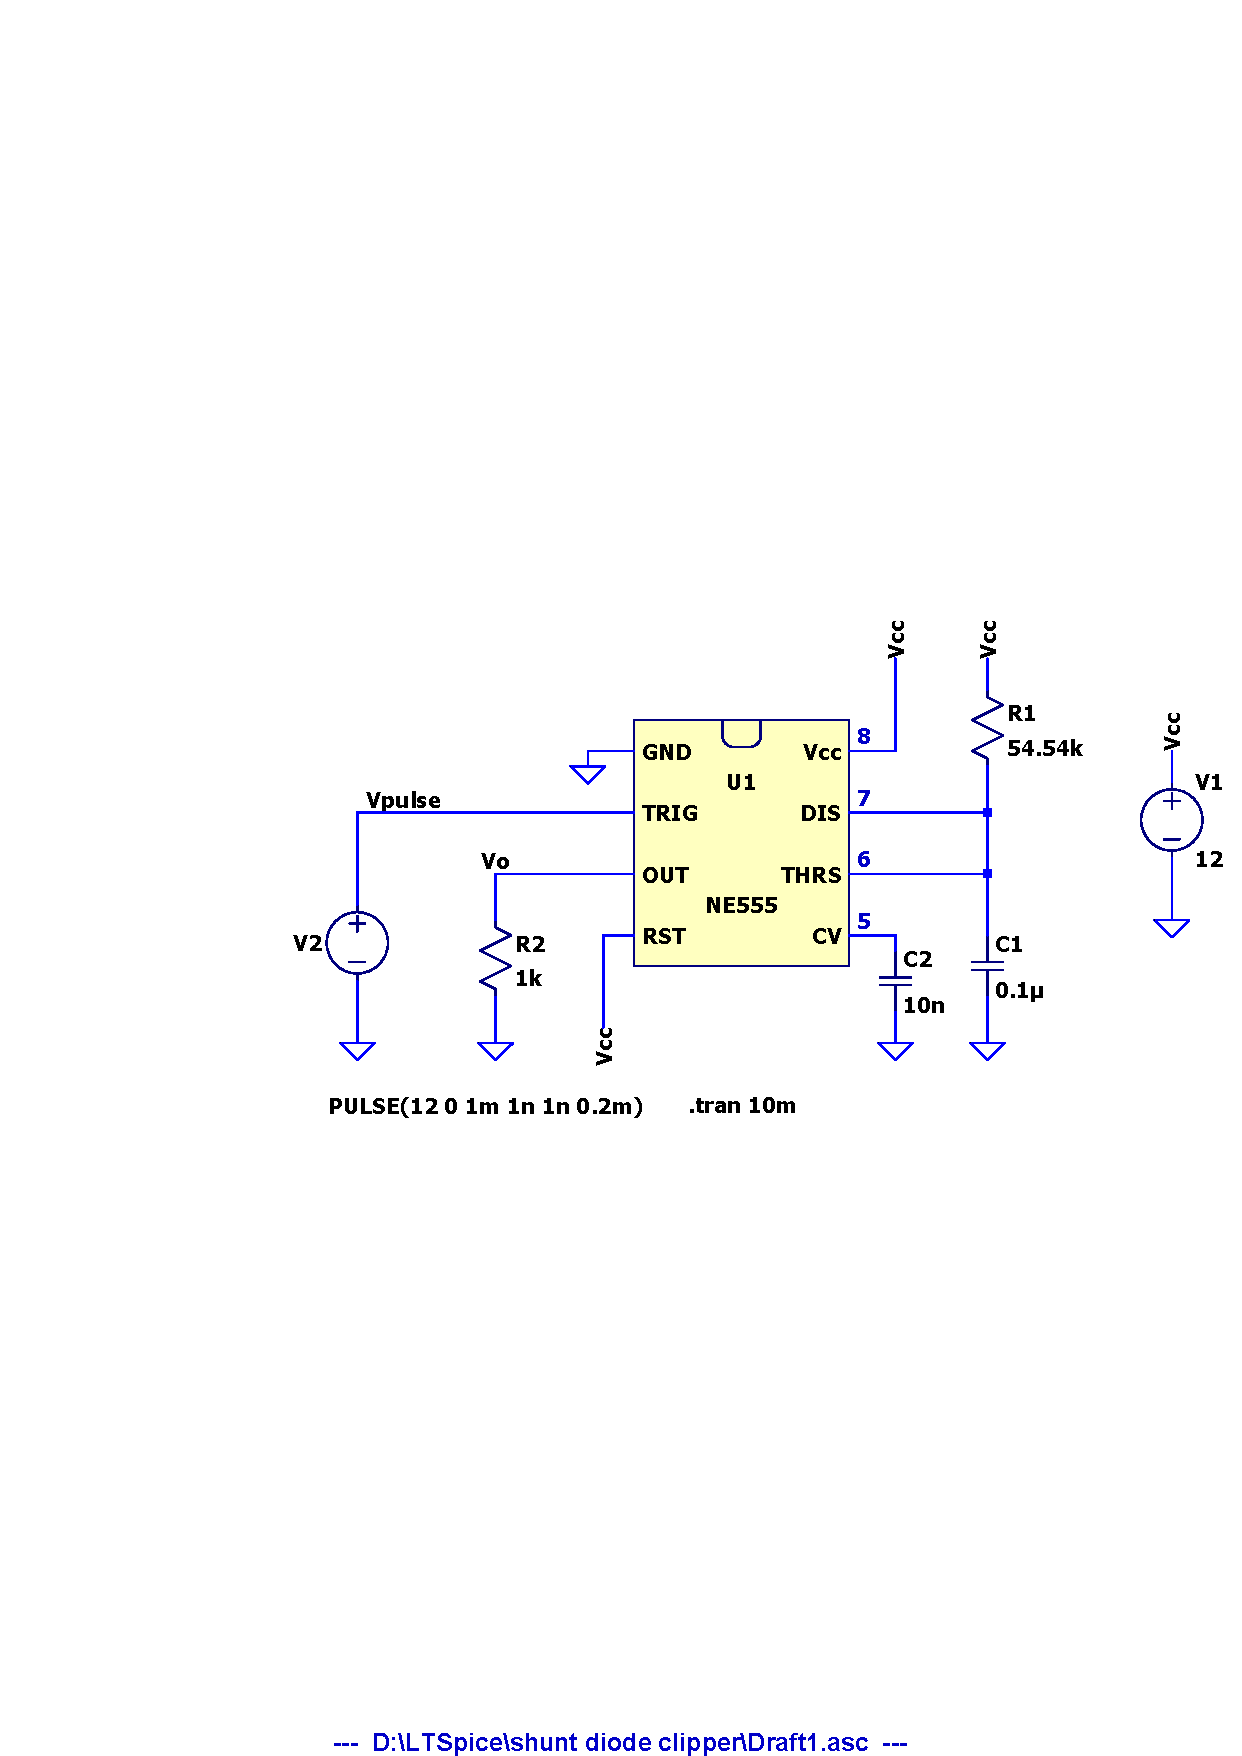
\includegraphics[clip, trim=5cm 10cm 0cm 10cm, scale=1]{Draft1}
\end{figure}

En la siguiente figura se muestra la gráfica del pulso de entrada (gráfica verde) y la señal de salida resultante (gráfica roja). Cada una de las gráficas tiene una serie de coordenadas (tiempo, voltaje). Para obtener el periodo de la señal de salida, simplemente restamos los dos periodos que se muestran, es decir:

\begin{align}
	t_p = \qty{6.9875909}{\milli \second} - \qty{1.0012837}{\milli \second} = \qty{5.9863072}{\milli \second} \approx \qty{6}{\milli \second} \nonumber
\end{align} 
\begin{figure}[H]
	\centering
	% trim=left botm right top
	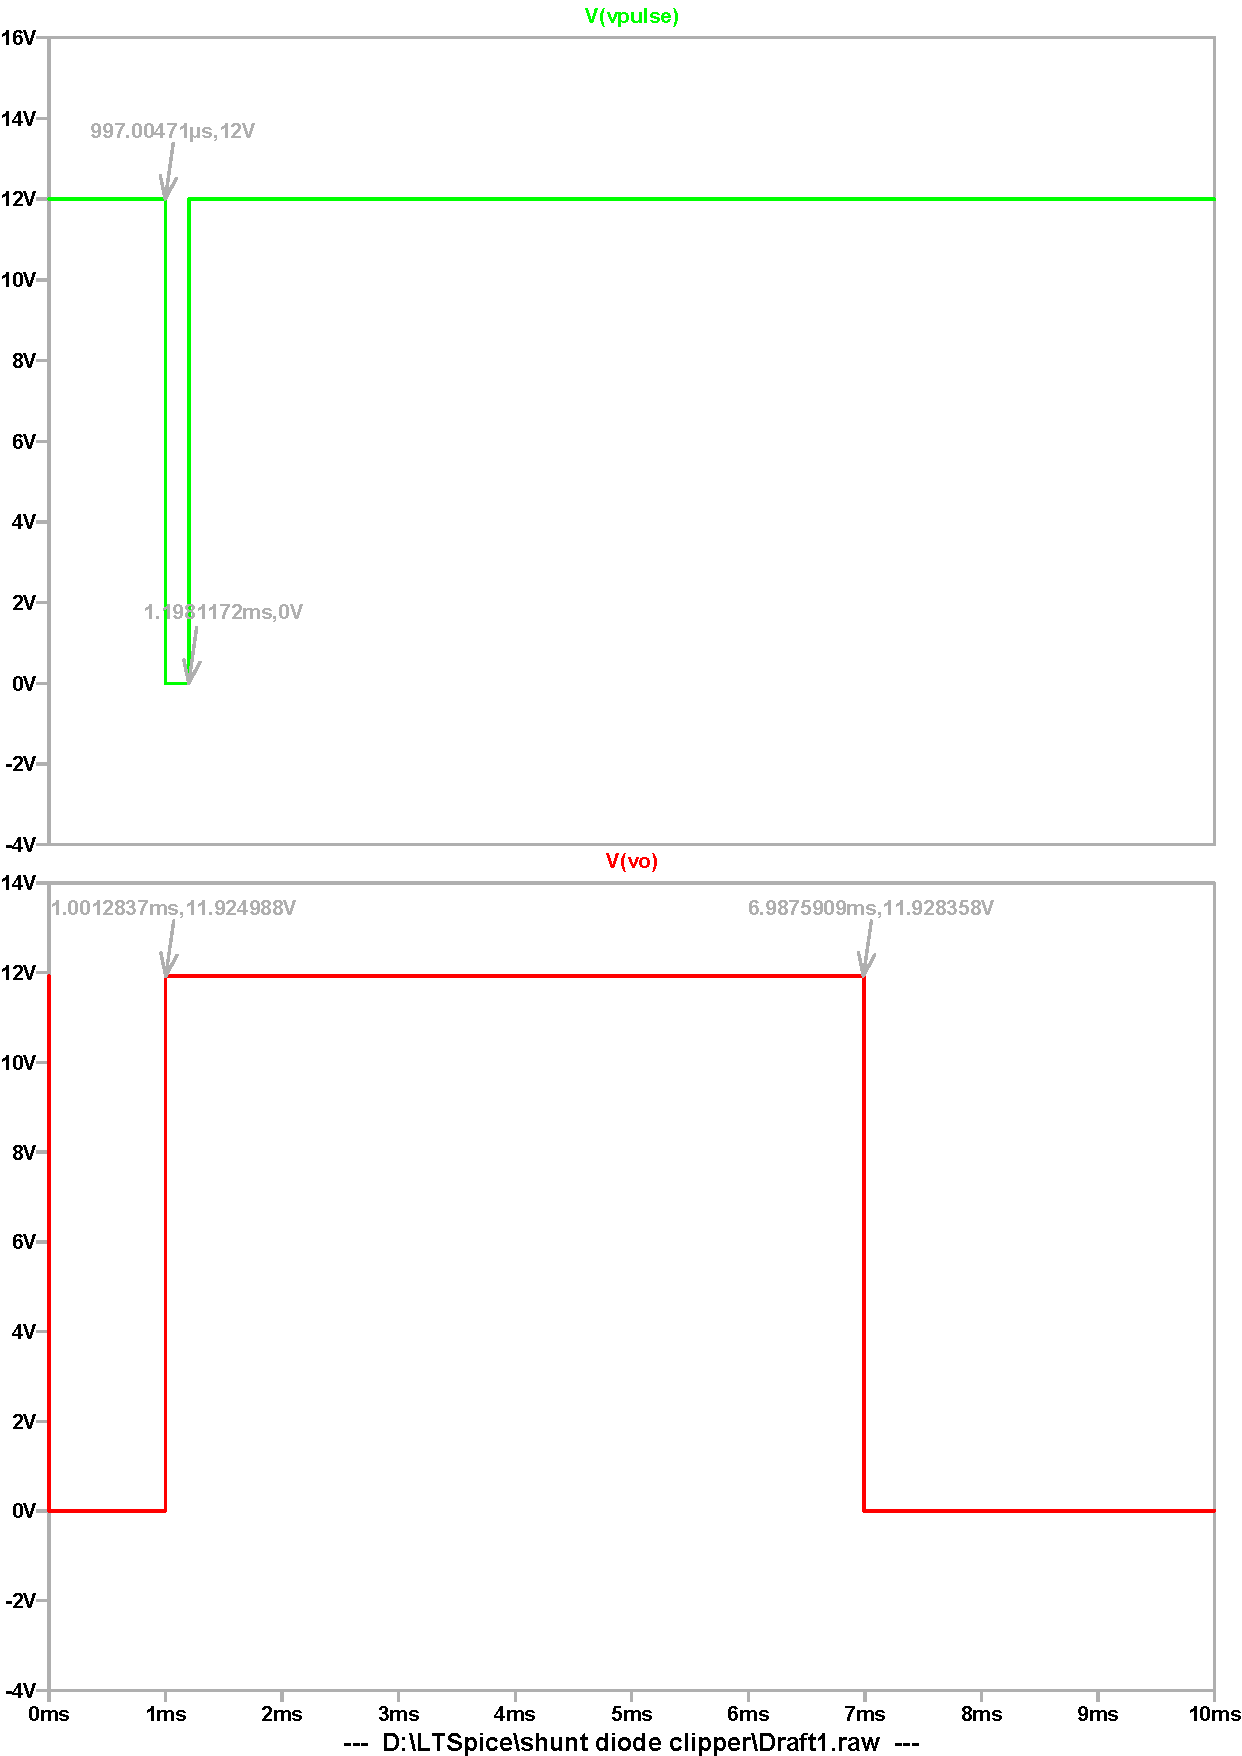
\includegraphics[clip, trim=0cm 0.5cm 0cm 0.1cm, width=\textwidth]{Draft2}
\end{figure}

\newpage

\section{Multivibrador astable}
Un multivibrador astable es un circuito generador de ondas rectangulares. Un $555$ conectado como multivibrador astable se muestra en la figura 10. La duración de los pulsos en estado $ALTO$ o $BAJO$ está determinado por los resistores $R_A$, $R_B$ y el capacitor $C$. Cuando la salida es $ALTA$, el capacitor $C_1$ intenta a cargarse hasta $V_{cc}$ a través de $R_A$ y $R_B$. Tan pronto como el voltaje en el capacitor iguala a $\frac{2V_{cc}}{3}$, la salida conmuta a un estado $BAJO$ y el capacitor $C_1$ se descargará a través de $R_B$ y el circuito interno del \textit{timer}.

\begin{figure}[H]
	\centering	
	\begin{tikzpicture}[scale=0.7, transform shape]
		\ctikzset{muxdemux/inner label font=\small}
		\ctikzset{muxdemux/outer label font={\small\color{blue}}}
		\tikzset{ic555/.style={muxdemux,
				muxdemux def={Lh=10, NL=7, Rh=10, NR=1, NB=2, w=6, NT=2}, %Lh = Left height, Rh = Right Heigh, w = width, NL = number of pin on the left, NR, number of pín on the right, NB = number of pins on the bottom 
				muxdemux label={L2=Discharge, L5=Trigger, L6=Threshold, R1=Out,
					T1={\ctikztextnot{RST}}, T2=VCC,  B1=GND, B2=Control, 
					LU2=7, LU5=6, LU6=2, TL1=8, TL2=4, RU1=3, BL1=1, BL2=5},
				external pins width=0.4,
				draw only left pins={2,5,6},
				circuitikz/muxdemuxes/fill=blue!10}
		}
		\node [ic555, font=\small\ttfamily,align=center](A) at (0,0) {LM555};
		\draw (A.lpin 2) to[short] ++(-1,0) coordinate (p1);
		\draw (A.tpin 2) to[short] ++(0,1) coordinate (t2); %top pin2
		\draw (p1) to[R, l=$R_1$] (p1 |- t2) coordinate (r1) to [short] (t2);
		\draw (A.tpin 1) to[short, -*] ++(0,1) to[short] ++(0,0.2) node[vcc](VCC){$+V_{CC}$};
		\draw (A.lpin 5) to[short] ++(-1,0) coordinate (p6);
		\draw (p1) to[R, l_=$R_2$, *-*] (p6);
		\draw (A.lpin 6) to[short, -*] ++(-1,0) coordinate (p2);
		\draw (p2) to[short] (p6);
		\draw (p2) to[cC, l_=$C_1$] ++(0,-3) coordinate (c1);
		\draw (A.bpin 1) to[short, -*] (c1 -| A.bpin 1) coordinate (pgnd);
		\draw (A.bpin 2) to[cC, l=$C_2$] (c1 -| A.bpin 2) --(pgnd);
		\draw (c1) to[short] (pgnd) node[ground]{};
		\draw (A.rpin 1) to[short, -o] ++(0.5,0);
		
		\pgfplotsset{width=9cm,height=5cm,compat=1.18}
		\begin{axis}[xshift=6cm,
			yshift=0cm,
			clip=false,
			axis y line=left,
			axis x line=middle,
			xlabel=$t$,
			ylabel=$v_O$, 
			axis y line= center,
			xmin=0,xmax=5,
			ymin=0,ymax=1.5,
			xtick={0},
			xticklabels={$$},
			ytick={-1,1},
			yticklabels={$V_{EE}$,$V_{CC}$},
			]
			\addplot+[line width=1pt,mark=none,const plot]
			coordinates {(0,1) (1.2,1) (1.2, 0) (2.2, 0) (2.2, 1) (3.4, 1) (3.4, 0) (4.4, 0) (4.4, 1) (4.8, 1)};
			\draw[|Stealth-] (2.2,1.2) node[right=13mm]{$T$} -- (3,1.2);
			\draw[|Stealth-] (4.4,1.2) -- (3.5,1.2);
			\addplot[color = black, dashed, thick] coordinates {(1.2,0) (1.2,-1.75)}; %vertical1
			\addplot[color = black, dashed, thick] coordinates {(2.2,0) (2.2,-1.75)}; %vertical1
			\addplot[color = black, dashed, thick] coordinates {(3.4,0) (3.4,-1.75)}; %vertical1
			\addplot[color = black, dashed, thick] coordinates {(4.4,0) (4.4,-1.75)}; %vertical1
		\end{axis}
		
		\pgfplotsset{width=9cm,compat=1.18}
		\begin{axis}[xshift=6cm,
			yshift=-4cm,
			clip=false,
			axis y line=left,
			axis x line=middle,
			xlabel=$t$,
			ylabel=$V_c$, 
			axis y line= center,
			xmin=0,xmax=5,
			ymin=0,ymax=1.5,
			xtick={0},
			xticklabels={$$},
			ytick={0.5, 1},
			yticklabels={$\frac{V_{cc}}{3}$,$\frac{2V_{cc}}{3}$},
			]
			\addplot[smooth, magenta,thick, mark=none, domain=0:1.2, samples=200] {1.5- exp(-(0.6*x)};
			\addplot[smooth, magenta,thick, mark=none, domain=1.2:2.2, samples=200] {exp(-0.7*(x-1.2))};
			\addplot[smooth, magenta,thick, mark=none, domain=2.2:3.4, samples=200] {1.5- exp(-(0.6*(x- 2.2))};
			\addplot[smooth, magenta,thick, mark=none, domain=3.4:4.4, samples=200] {exp(-0.7*(x-3.4))};
			\addplot[smooth, magenta,thick, mark=none, domain=4.4:4.8, samples=200] {1.5- exp(-(0.6*(x- 4.4))};
			\addplot[color = black, dashed, thick] coordinates {(0, 0.5) (2.2,0.5)}; %vertical1
			\addplot[color = black, dashed, thick] coordinates {(0, 1) (1.2,1)}; %vertical1
			\draw[|Stealth-] (2.2,1.2) node[right=6mm]{$t_c$} -- (2.6,1.2);
			\draw[|Stealth-] (3.4,1.2) -- (2.9,1.2);
			\draw[|Stealth-] (3.4,1.2) node[right=5mm]{$t_d$} -- (3.7,1.2);
			\draw[|Stealth-] (4.4,1.2) -- (4.1,1.2);
		\end{axis}
	\end{tikzpicture}
	\caption{Multivibrador astable. (a) circuito, (b) Formas de onda}	
	\label{fig:figura10}
\end{figure}

\noindent Inicialmente el capacitor se encuentra descargado, por lo que el comparador $CM_1$ envía un estado $BAJO$ a la entrada de $R$ del \textit{latch} y el comparador $CM_2$ envía un estado $ALTO$ a la entrada $S$ del mismo (figura 11).

\begin{figure}[H]
	\centering
	\scalebox{.9}{	
		\begin{tikzpicture}[scale=0.8]
			\ctikzset{bipoles/thickness=4}
			\ctikzset{monopoles/vcc/arrow={Stealth[width=6pt,length=9pt]}}
			\ctikzset{monopoles/vee/arrow={Stealth[width=6pt,length=9pt]}}
			\node[flipflop myRS] (RS) at (0,0){};
			\draw (RS.pin 1) node[left=2.2mm, above]{$BAJO$} to [short] ++(-1,0)  -- ++(0,1) -- ++(-1,0) coordinate (p1);
			\draw (p1) node[op amp, noinv input up, anchor=out](OA1){$CM_1$};
			\draw (RS.pin 3) to[short] ++(-1,0) node[right=5.5mm, below]{$ALTO$} -- ++(0,-1) -- ++(-1,0) coordinate (p2);
			\draw (p2) node[op amp, noinv input up, anchor=out](OA2){$CM_2$};
			\draw (OA1.-) to[short] ++(-1,0) coordinate (p3);
			\draw (OA2.+) to[short] ++(-1,0) coordinate (p4);
			\draw (p3) to[R, *-*, l=$R$] (p4);
			\draw (RS.pin 4) node[right=5mm, above]{$BAJO$} to[short] ++(2,0) to[short] ++(0,5)  to[R] ++(-3,0) to[short] ++(-1.5,0) coordinate(p5);
			\draw (p5) node[npn, anchor=B, xscale=-1](Q){}	;
			\draw (RS.pin 6) node[right=5mm, above]{$ALTO$} to[short, -o] ++(4,0) node[right]{$Out$} node[below]{$3$};
			\draw (p4) to[short] ++(0,-1) to[R, l=$R$] ++(0,-3) coordinate(x3) to[short] ++(0,-0.15) node[ground]{};
			\draw (OA2.-) to[short] ++(-4,0) coordinate (c1) node[above right]{$(2)$} to[cC, l_=$C_1$, *-, v^=$\qty{0}{\volt}$] ++(0,-3) node[ground]{};
			\draw (OA1.+) to[short] ++(-2,0) to[short] ++(0,-4) to[short] ++(-2,0) coordinate (c2) node[above right]{$(6)$} to[short] (c1);
			\draw (Q.C) to[short] ++(0,0.4) coordinate (p7);
			\draw (Q.E) node[ground]{};
			\draw (p3) to[R, l_=$R$] ++(0,5) coordinate(p8) node[vcc](VCC){$+V_{CC}$};
			\draw (RS.up) coordinate(x1) to[short] (x1 |- p8) node[vcc](VCC){$+V_{CC}$} coordinate(x2);
			\draw[black, dashed, thick] (-9,5.5) rectangle (4.5,-6.7);
			\draw (Q.B) node[left=7mm]{$Q_1$} node[right=1mm, above]{$OFF$};
			\draw (c2) to[R, *-*, l=$R_B$] ++(0,4) coordinate (c4) node[above right]{$(7)$};
			\draw (p7) to[short] ++(-7.5,0) coordinate (c5);
			\draw (c5) to[short] (c4 -| c5) -- (c4);
			\draw (c4) to[R, l=$R_A$] ++(0,3.75) node[vcc](VCC){$+V_{CC}$};
			\draw[-Stealth](-11,7) -- ++(0,-1) coordinate (arr1);
			\draw[-Stealth] (arr1)++(0,-2) -- ++(0,-1) coordinate (arr2);
			\draw[-Stealth] (arr2)++(0,-0.5) -- ++(0,-1) coordinate (arr3);
			\draw[-Stealth] (arr3)++(0,-2) -- ++(0,-1) coordinate (arr4);
			\draw[-Stealth] (arr4)++(0,-0.5) -- ++(0,-1) coordinate (arr5);
			\draw[-Stealth] (arr5)++(0,-2) -- ++(0,-1) coordinate (arr6);
	\end{tikzpicture}}
	\caption{Estado inicial del multivibrador astable cuando el capacitor está descargado.}	
	\label{fig:figura11}
\end{figure}

\noindent La combinación $(R = 0, S = 1)$ establece al \textit{latch} en estado $SET$ poniendo la salida $Q$ del \textit{latch} en estado $ALTO$ y además coloca al transistor $Q_1$ en estado de corte, permitiendo que la corriente fluya a través de las resistencias $R_A$ y $R_B$, haciendo que el capacitor se cargue.

\noindent Cuando el voltaje en el capacitor sobrepasa el voltaje $\frac{V_{cc}}{3}$ (figura 12), la salida del comparador $CM_2$ enviará un estado $BAJO$ a la entrada $S$ del \textit{latch}, mientras que el comparador $CM_1$ permanece sin cambios, por lo tanto, la combinación $(R = 0, S = 0)$ hace que el \textit{latch} permanezca sin cambios, por lo que el capacitor continuará cargándose.

\begin{figure}[H]
	\centering
	\scalebox{.9}{	
		\begin{tikzpicture}[scale=0.8]
			\ctikzset{bipoles/thickness=4}
			\ctikzset{monopoles/vcc/arrow={Stealth[width=6pt,length=9pt]}}
			\ctikzset{monopoles/vee/arrow={Stealth[width=6pt,length=9pt]}}
			\node[flipflop myRS] (RS) at (0,0){};
			\draw (RS.pin 1) node[left=2.2mm, above]{$BAJO$} to [short] ++(-1,0)  -- ++(0,1) -- ++(-1,0) coordinate (p1);
			\draw (p1) node[op amp, noinv input up, anchor=out](OA1){$CM_1$};
			\draw (RS.pin 3) to[short] ++(-1,0) node[right=5.5mm, below]{$BAJO$} -- ++(0,-1) -- ++(-1,0) coordinate (p2);
			\draw (p2) node[op amp, noinv input up, anchor=out](OA2){$CM_2$};
			\draw (OA1.-) to[short] ++(-1,0) coordinate (p3);
			\draw (OA2.+) to[short] ++(-1,0) coordinate (p4);
			\draw (p3) to[R, *-*, l=$R$] (p4);
			\draw (RS.pin 4) node[right=5mm, above]{$BAJO$} to[short] ++(2,0) to[short] ++(0,5)  to[R] ++(-3,0) to[short] ++(-1.5,0) coordinate(p5);
			\draw (p5) node[npn, anchor=B, xscale=-1](Q){}	;
			\draw (RS.pin 6) node[right=5mm, above]{$ALTO$} to[short, -o] ++(4,0) node[right]{$Out$} node[below]{$3$};
			\draw (p4) to[short] ++(0,-1) to[R, l=$R$] ++(0,-3) coordinate(x3) to[short] ++(0,-0.15) node[ground]{};
			\draw (OA2.-) to[short] ++(-4,0) coordinate (c1) node[above right]{$(2)$} to[cC, l_=$C_1$, *-, v^=$\frac{V_{cc}}{3}$] ++(0,-3) node[ground]{};
			\draw (OA1.+) to[short] ++(-2,0) to[short] ++(0,-4) to[short] ++(-2,0) coordinate (c2) node[above right]{$(6)$} to[short] (c1);
			\draw (Q.C) to[short] ++(0,0.4) coordinate (p7);
			\draw (Q.E) node[ground]{};
			\draw (p3) to[R, l_=$R$] ++(0,5) coordinate(p8) node[vcc](VCC){$+V_{CC}$};
			\draw (RS.up) coordinate(x1) to[short] (x1 |- p8) node[vcc](VCC){$+V_{CC}$} coordinate(x2);
			\draw[black, dashed, thick] (-9,5.5) rectangle (4.5,-6.7);
			\draw (Q.B) node[left=7mm]{$Q_1$} node[right=1mm, above]{$OFF$};
			\draw (c2) to[R, *-*, l=$R_B$] ++(0,4) coordinate (c4) node[above right]{$(7)$};
			\draw (p7) to[short] ++(-7.5,0) coordinate (c5);
			\draw (c5) to[short] (c4 -| c5) -- (c4);
			\draw (c4) to[R, l=$R_A$] ++(0,3.75) node[vcc](VCC){$+V_{CC}$};
			\draw[-Stealth](-11,7) -- ++(0,-1) coordinate (arr1);
			\draw[-Stealth] (arr1)++(0,-2) -- ++(0,-1) coordinate (arr2);
			\draw[-Stealth] (arr2)++(0,-0.5) -- ++(0,-1) coordinate (arr3);
			\draw[-Stealth] (arr3)++(0,-2) -- ++(0,-1) coordinate (arr4);
			\draw[-Stealth] (arr4)++(0,-0.5) -- ++(0,-1) coordinate (arr5);
			\draw[-Stealth] (arr5)++(0,-2) -- ++(0,-1) coordinate (arr6);
	\end{tikzpicture}}
	\caption{Estado del circuito cuando el capacitor alcanza un voltaje de $\frac{V_{cc}}{3}$.}	
	\label{fig:figura12}
\end{figure}

Ahora,cuando el capacitor sobrepase un voltaje de $\frac{2V_{cc}}{3}$, el comparador $CM_1$ enviará un estado $ALTO$ a la entrada $R$ del \textit{latch} y un estado $BAJO$ a la entrada $S$ del mismo, por lo tanto, la combinación $(R = 1, S = 0)$ establecerá al \textit{latch} en un estado de $RESET$ haciendo que la salida $Q$ de éste envíe un estado $BAJO$ y haciendo que el transistor $Q_1$ entre en estado de saturación, por lo que el capacitor se descargará gradualmente a través de $R_B$.


\begin{figure}[H]
	\centering
	\scalebox{.9}{	
		\begin{tikzpicture}[scale=0.8]
			\ctikzset{bipoles/thickness=4}
			\ctikzset{monopoles/vcc/arrow={Stealth[width=6pt,length=9pt]}}
			\ctikzset{monopoles/vee/arrow={Stealth[width=6pt,length=9pt]}}
			\node[flipflop myRS] (RS) at (0,0){};
			\draw (RS.pin 1) node[left=2.2mm, above]{$ALTO$} to [short] ++(-1,0)  -- ++(0,1) -- ++(-1,0) coordinate (p1);
			\draw (p1) node[op amp, noinv input up, anchor=out](OA1){$CM_1$};
			\draw (RS.pin 3) to[short] ++(-1,0) node[right=5.5mm, below]{$BAJO$} -- ++(0,-1) -- ++(-1,0) coordinate (p2);
			\draw (p2) node[op amp, noinv input up, anchor=out](OA2){$CM_2$};
			\draw (OA1.-) to[short] ++(-1,0) coordinate (p3);
			\draw (OA2.+) to[short] ++(-1,0) coordinate (p4);
			\draw (p3) to[R, *-*, l=$R$] (p4);
			\draw (RS.pin 4) node[right=5mm, above]{$ALTO$} to[short] ++(2,0) to[short] ++(0,5)  to[R] ++(-3,0) to[short] ++(-1.5,0) coordinate(p5);
			\draw (p5) node[npn, anchor=B, xscale=-1](Q){}	;
			\draw (RS.pin 6) node[right=5mm, above]{$BAJO$} to[short, -o] ++(4,0) node[right]{$Out$} node[below]{$3$};
			\draw (p4) to[short] ++(0,-1) to[R, l=$R$] ++(0,-3) coordinate(x3) to[short] ++(0,-0.15) node[ground]{};
			\draw (OA2.-) to[short] ++(-4,0) coordinate (c1) node[above right]{$(2)$} to[cC, l_=$C_1$, *-, v^=$\frac{V_{cc}}{3}$] ++(0,-3) node[ground]{};
			\draw (OA1.+) to[short] ++(-2,0) to[short] ++(0,-4) to[short] ++(-2,0) coordinate (c2) node[above right]{$(6)$} to[short] (c1);
			\draw (Q.C) to[short] ++(0,0.4) coordinate (p7);
			\draw (Q.E) node[ground]{};
			\draw (p3) to[R, l_=$R$] ++(0,5) coordinate(p8) node[vcc](VCC){$+V_{CC}$};
			\draw (RS.up) coordinate(x1) to[short] (x1 |- p8) node[vcc](VCC){$+V_{CC}$} coordinate(x2);
			\draw[black, dashed, thick] (-9,5.5) rectangle (4.5,-6.7);
			\draw (Q.B) node[left=7mm]{$Q_1$} node[right=1mm, above]{$OFF$};
			\draw (c2) to[R, *-*, l=$R_B$] ++(0,4) coordinate (c4) node[above right]{$(7)$};
			\draw (p7) to[short] ++(-7.5,0) coordinate (c5);
			\draw (c5) to[short] (c4 -| c5) -- (c4);
			\draw (c4) to[R, l=$R_A$] ++(0,3.75) node[vcc](VCC){$+V_{CC}$};
			\draw[Stealth-] (arr2)++(0,-0.5) -- ++(0,-1) coordinate (arr3);
			\draw[Stealth-] (arr3)++(0,-2) -- ++(0,-1) coordinate (arr4);
			\draw[Stealth-] (arr4)++(0,-0.5) -- ++(0,-1) coordinate (arr5);
			\draw[Stealth-] (arr5)++(0,-2) -- ++(0,-1) coordinate (arr6);
			\draw[-Stealth] (c4)++(0.1,-0.2) -- ++(1,0) coordinate (arr7);
			\draw[-Stealth] (arr7)++(0.1,0) -- ++(0,1) coordinate (arr8);
			\draw[-Stealth] (arr8)++(0,0.5) -- ++(0,1) coordinate (arr9);
			\draw[-Stealth] (arr9)++(0.5,0) -- ++(1,0) coordinate (arr10);
			\draw[-Stealth] (arr10)++(0.5,0) -- ++(1,0) coordinate (arr11);
			\draw[-Stealth] (arr11)++(0.5,0) -- ++(1,0) coordinate (arr12);
			\draw[-Stealth] (arr12)++(0.5,0) -- ++(1,0) coordinate (arr13);
			\draw[-Stealth] (arr13)++(0,-0.5) -- ++(0,-1) coordinate (arr14);
	\end{tikzpicture}}
	\caption{Estado del circuito cuando el capacitor alcanza un voltaje de $\frac{2V_{cc}}{3}$.}	
	\label{fig:figura13}
\end{figure}

\noindent El capacitor es cargado y descargado periódicamente entre $\frac{2V_{cc}}{3}$ y $\frac{V_{cc}}{3}$. Asumiendo que el voltaje inicial en el capacitor es de $V_c(0) = \frac{V_{cc}}{3}$, el circuito equivalente durante el periodo de carga se muestra en la figura 14.

\subsection*{Tiempo de carga}
\begin{figure}[H]
	\centering	
	\begin{tikzpicture}[scale=0.8]
		\ctikzset{bipoles/thickness=4}
		\ctikzset{monopoles/vcc/arrow={Stealth[width=6pt,length=9pt]}}
		\ctikzset{monopoles/vee/arrow={Stealth[width=6pt,length=9pt]}}
		\draw (0,0) coordinate (p1) to[cC, l=$C_1$, v={$V_c(0) = \frac{V_{cc}}{3}$}] ++(0,-4) coordinate (p2);
		\draw (p1) to[R, l=$R_B$] ++(4, 0) to [R, l=$R_A$, -o] ++(4, 0) coordinate (e1);
		\draw (p2) to[short, -o] (p2 -| e1);
		\draw (e1) to[open, v=$V_{cc}$] ++(0,-4); 
	\end{tikzpicture}
	\caption{Circuito equivalente para el tiempo de carga.}	
	\label{fig:figura14}
\end{figure}

Nuevamente, la ecuación general de voltaje en el capacitor se expresa como

\begin{align}
	v_c(t) = v(\infty) + \left[ v(0) - v(\infty) \right]e^{-\frac{t}{\tau}} 
\end{align}

Para el tiempo de carga, tenemos los siguientes valores:

\begin{subequations}
\begin{align}
	v(0) = \frac{V_{cc}}{3} \label{second:a} \\
	v(\infty) = V_{cc} \label{second:b}
\end{align}
\end{subequations}

Al sustituir la ecuación 13a y 13b en la ecuación (12) obtenemos

\begin{align}
	v_c(t) &= V_{cc} + \left[ \frac{V_{cc}}{3} - V_{cc} \right]   e^{-\frac{t}{\tau}} \nonumber \\
	v_c(t) &= V_{cc} - \frac{2V_{cc}}{3}e^{-\frac{t}{\tau}}
\end{align}

Donde 
\begin{align}
	\tau = (R_A + R_B)C_1
\end{align}

\noindent El capacitor $C_1$ se cargará a través de la combinación en serie de $R_A$ y $R_B$, y el voltaje en sus termianles se elevará en forma exponencial. El circuito estará en un nivel alto hasta que $V_c(t)$ alcance el voltaje de umbral del comparador $CM_1$ $(\frac{2V_{cc}}{3})$. Al sustituir este valor en la ecuación (14) obtenemos

\begin{align}
	\frac{2V_{cc}}{3} = V_{cc} - \frac{2V_{cc}}{3}e^{-\frac{t}{(R_A + R_B)C_1}}
\end{align}

\noindent Reordenamos términos para simplificar:

\begin{align}
	\frac{2V_{cc}}{3} - V_{cc}  &= -\frac{2V_{cc}}{3}e^{-\frac{t}{(R_A + R_B)C_1}} \nonumber \\
	-\frac{V_{cc}}{3} &= -\frac{2V_{cc}}{3}e^{-\frac{t}{(R_A + R_B)C_1}} \nonumber \\
	1 &= 2e^{-\frac{t}{(R_A + R_B)C_1}} \nonumber \\
	\frac{1}{2} &= e^{-\frac{t}{(R_A + R_B)C_1}} \nonumber \\
	2 &= e^{\frac{t}{(R_A + R_B)C_1}} \nonumber \\
	\ln(2) &= \ln \left[ e^{\frac{t}{(R_A + R_B)C_1}} \right]  \nonumber \\
	\ln(2) &= \frac{t}{(R_A + R_B)C_1}  
\end{align}

\noindent De esta manera, el tiempo de carga $t_c$ está representado por la siguiente expresión:

\begin{tcolorbox}[colback=red!5!white,colframe=red!75!black,arc=0mm,boxrule=0mm,width=(\linewidth+0.5cm)]
\begin{equation}
	t_c = (R_A + R_B)C_1 \ln(2)
\end{equation}
\end{tcolorbox}


\noindent Para obtener la corriente durante el tiempo de carga empleamos la relación $i-v$ del capacitor, la cual se representa como

\begin{align}
	i_{C_1}(t) = C \frac{dv_c(t)}{dt}
\end{align}

\noindent Sustituimos la ecuación (14) en (19) y resolvemos

\begin{align}
	i_{C_1}(t) = C \frac{d}{dt} \left[ V_{cc} - \frac{2V_{cc}}{3}e^{-\frac{t}{\tau}} \right]
\end{align}

\noindent O bien

\begin{align}
	i_{C_1}(t) = \frac{2V_{cc}}{3(R_A + R_B)} e^{-\frac{t}{\tau}} = i_{R_A}(t) = i_{R_B}(t)
\end{align}

\noindent La corriente inicial en $t=0$ es

\begin{align}
	i_{C_1}(t=0) = i_{R_A}(t) = i_{R_B}(t) =  \frac{2V_{cc}}{3(R_A + R_B)}
\end{align}

\noindent La corriente en $t=tc$ es

\begin{align}
	i_{C_1}(t) = \frac{2V_{cc}}{3(R_A + R_B)} e^{ -\frac{(R_A + R_B)C_1 \ln(2)}{(R_A + R_B)C_1} } = \frac{2V_{cc}}{3(R_A + R_B)} e^{ -\ln(2) } =
\end{align}

O bien

\begin{align}
	i_{C_1}(t=t_c) = \frac{2V_{cc}}{6(R_A + R_B)}
\end{align}

\noindent Por lo tanto

\begin{tcolorbox}[colback=red!5!white,colframe=red!75!black,arc=0mm,boxrule=0mm,width=(\linewidth+0.5cm)]
	\begin{align}
		i_{C_1}(t) = i_{R_A}(t) = i_{R_B}(t) = \frac{2V_{cc}}{3(R_A + R_B)} e^{-\frac{t}{\tau}},  \quad 0 \leq t \leq t_c = 
		\begin{cases}
			\frac{2V_{cc}}{3(R_A + R_B)}, \quad t = 0 \\
			\frac{2V_{cc}}{6(R_A + R_B)}, \quad t = t_c
		\end{cases}	
	\end{align}
\end{tcolorbox}

\subsection*{Tiempo de descarga}
Durante el tiempo de descarga, el capacitor C se descarga de $\frac{2V_{cc}}{3}$ a $\frac{V_{cc}}{3}$ a través de $R_B$ como se muestra en la figura 13. El circuito equivalente de descarga se muestra en la figura 14.

\begin{figure}[H]
	\centering	
	\begin{tikzpicture}[scale=0.8]
		\ctikzset{bipoles/thickness=4}
		\ctikzset{monopoles/vcc/arrow={Stealth[width=6pt,length=9pt]}}
		\ctikzset{monopoles/vee/arrow={Stealth[width=6pt,length=9pt]}}
		\draw (0,0) coordinate (p1) to[cC, l=$C_1$, v={$V_c(0) = \frac{2V_{cc}}{3}$}] ++(0,-4) coordinate (p2);
		\draw (p1) to[R, l=$R_B$] ++(4, 0) coordinate (e1) -- ++(0,-4);
		\draw (p2) to[short] (p2 -| e1);
	\end{tikzpicture}
	\caption{Circuito equivalente para el tiempo de descarga.}	
	\label{fig:figura15}
\end{figure}

Para el tiempo de descarga, tenemos los siguientes valores:

\begin{subequations}
	\begin{align}
		v(0) &= \frac{2V_{cc}}{3} \label{second:a} \\
		v(\infty) &= 0 \label{second:b}
	\end{align}
\end{subequations}

La sustitución de los valores dados en la ecuación 26 en la ecuación 12 produce
\begin{align}
	v_c(t) &= 0 + \left[ \frac{2V_{cc}}{3} - 0 \right] e^{-\frac{t}{\tau}} \nonumber \\
	v_c(t) &= \frac{2V_{cc}}{3} e^{-\frac{t}{\tau}}
\end{align}

Donde

\begin{align}
	\tau = R_BC_1
\end{align}

El capacitor se descargará hasta que alcance un voltaje de $\frac{V_{cc}}{3}$, así

\begin{align}
	\frac{V_{cc}}{3} &= \frac{2V_{cc}}{3} e^{-\frac{t}{\tau}} \nonumber \\
	1 &= 2 e^{-\frac{t}{\tau}} \nonumber \\
	\frac{1}{2} &= e^{-\frac{t}{\tau}} \nonumber \\
	2 &= e^{-\frac{t}{\tau}}
\end{align}

\begin{align}
	\ln (2) = \ln \left( e^{\frac{t}{\tau}} \right) \nonumber \\
	t = \tau \ln (2) \nonumber
\end{align}

Así, el tiempo de descarga está representando por


\begin{tcolorbox}[colback=red!5!white,colframe=red!75!black,arc=0mm,boxrule=0mm,width=(\linewidth+0.5cm)]
	\begin{equation}
		t_d = R_BC_1 \ln (2)
	\end{equation}
\end{tcolorbox}

Nuevamente, calculamos la corriente que circula por el capacitor, que será la misma corriente que circule por el resistor $R_B$

\begin{align}
	i_{C_1}(t) = i_{R_B}(t) = C \frac{dv_c(t)}{dt}  = C_1 \frac{d}{dt} \left[ \frac{2V_{cc}}{3} e^{-\frac{t}{\tau}} \right] = \frac{2C_1V_{cc}}{3} \left( -\frac{1}{R_BC_1} \right) e^{-\frac{t}{\tau}} \nonumber
\end{align}

\begin{align}
	i_{C_1}(t) = i_{R_B}(t) = -\frac{2V_{cc}}{3R_B}e^{-\frac{t}{\tau}}
\end{align}

La corriente inicical en el inicio del tiempo de descarga que denominaremos también como t=0 es:

\begin{align}
	i_{C_1}(t=0) =  -\frac{2V_{cc}}{3R_B} = i_{R_B}(t=0)
\end{align}

La corriente en $t=t_d$ es

\begin{align}
	i_{C_1}(t=t_d) = -\frac{2V_{cc}}{3R_B}e^{-\frac{R_BC_1\ln(2)}{R_BC_1}} = -\frac{2V_{cc}}{3R_B} e^{-\ln(2)} = -\frac{V_{cc}}{3R_B}
\end{align}

Así

\begin{tcolorbox}[colback=red!5!white,colframe=red!75!black,arc=0mm,boxrule=0mm,width=(\linewidth+0.5cm)]
	\begin{align}
		i_{C_1}(t) = i_{R_B}(t) = -\frac{2V_{cc}}{3R_B}e^{-\frac{t}{\tau}},  \quad tc \leq t \leq t_d = 
		\begin{cases}
			-\frac{2V_{cc}}{3R_B}, \quad t = tc \\
			-\frac{V_{cc}}{3R_B}, \quad t = t_d
		\end{cases}	
	\end{align}
\end{tcolorbox}

Como podemos observar de la figura 13, el capacitor se descarga a través de la resistencia $R_B$, esto gracias a que el transistor interno del dispositivo se encuentra en saturación, actuando como un interruptor cerrado. La resistencia $R_A$ no tiene un papel en la descarga del capacitor, sin embargo sí circula corriente por ella ya que también encuentra un camino de baja resistencia a través del transistor. Dicha corriente durante el tiempo de descarga es:

\begin{align}
	i_{R_A} = \frac{V_{cc}}{R_A}
\end{align}

La corriente que circula por los elementos a lo largo del periodo $T$ es

\begin{tcolorbox}[colback=red!5!white,colframe=red!75!black,arc=0mm,boxrule=0mm,width=(\linewidth+0.5cm)]
	\begin{align}
		i_{R_A}(t) = 
		\begin{cases}
			 \frac{2V_{cc}}{3(R_A + R_B)} e^{-\frac{t}{(R_A + R_B)C_1\ln(2)}}, &\quad 0 \leq t \leq  t_c \\
			-\frac{2V_{cc}}{3R_B}e^{-\frac{t}{R_BC_1}}, &\quad t_c \leq t \leq t_d
		\end{cases}	=
		\begin{cases}
			\frac{2V_{cc}}{3(R_A + R_B)}, &\quad t_c = 0 \\
			\frac{1V_{cc}}{3(R_A + R_B)}, &\quad t = t_c \\
			\frac{V_{cc}}{R_A}, &\quad t_c \leq t \leq t_d 
		\end{cases}
	\end{align}
\end{tcolorbox}

\begin{tcolorbox}[colback=red!5!white,colframe=red!75!black,arc=0mm,boxrule=0mm,width=(\linewidth+0.5cm)]
	\begin{align}
		i_{R_B}(t) = i_{C_1}(t)=
		\begin{cases}
			\frac{2V_{cc}}{3(R_A + R_B)} e^{-\frac{t}{(R_A + R_B)C_1\ln(2)}}, &\quad 0 \leq t \leq  t_c \\
			-\frac{2V_{cc}}{3R_B}e^{-\frac{t}{R_BC_1}}, &\quad t_c \leq t \leq t_d
		\end{cases}	=
		\begin{cases}
			\frac{2V_{cc}}{3(R_A + R_B)}, &\quad t_c = 0 \\
			\frac{1V_{cc}}{3(R_A + R_B)}, &\quad t = t_c^{-}  \\
			-\frac{2V_{cc}}{3R_B}, &\quad t = t_c^{+} \\
			-\frac{V_{cc}}{3R_B}, &\quad t = t_d
		\end{cases}
	\end{align}
\end{tcolorbox}

El periodo total del pulso de salida se obtiene de la suma de las ecuaciones (18) y (30), es decir

\begin{align}
	T = t_c + t_d = (R_A + R_B)C_1 \ln(2) + R_BC_1 \ln(2) = (R_A + 2R_B)C_1 \ln(2)
\end{align}

La frecuencia de la señal de salida es
\begin{tcolorbox}[colback=red!5!white,colframe=red!75!black,arc=0mm,boxrule=0mm,width=(\linewidth+0.5cm)]
	\begin{equation}
		f = \frac{1}{T} = \frac{1}{(R_A + 2R_B)C_1 \ln(2)}
	\end{equation}
\end{tcolorbox}

El ciclo de trabajo se define como la razón entre el tiempo de carga $t_c$ y el periodo $T$, es decir

\begin{align}
	D = \frac{t_c}{T} = \frac{(R_A + R_B)C_1\ln(2)}{(R_A + 2R_B)C_1\ln(2)} = \frac{R_A + R_B}{R_A + 2R_B} = 1 - \frac{1}{2 + \frac{R_A}{R_B}}
\end{align}

Al observar la ecuación (40) notamos que el ciclo de trabajo sólo puede ser mayor al 50\%, es decir, no podemos hacer que el tiempo de carga sera menor al tiempo de descarga. Para poder hacer que el ciclo de trabajo varíe entre el 0 y el 100\% debemos agregar simplemente un par de diodos al circuito, sin embargo, el análisis de este nuevo circuito se tratará más adelante con mayor detalle.

Al despejar $t_c$ de la ecuación (40) obtenemos

\begin{align}
	t_c = DT
\end{align}

Si sustituimos la ecuación (41) en (38) obtenemos

\begin{align}
	T = DT + t_d
\end{align}

Si despejamos el tiempo de descarga de la ecuación (42) obtenemos

\begin{align}
	t_d = T(1 - D)
\end{align}

Para encontrar el valor del resistor $R_B$ despejamos este ultimo de la ecuación (30), es decir

\begin{align}
	R_B = \frac{t_d}{C_1 \ln(2)}
\end{align}

Ahora despejamos $R_A$ de la ecuación (18)

\begin{align}
	R_A = \frac{t_c}{C_1 \ln(2)} - R_B
\end{align}

\subsection*{Ejemplo 1}
Diseñe un multivibrador astable que opere con un ciclo de trabajo $D=63\%$ a una frecuencia $f=\qty{2.65}{\kilo\hertz}$

\subsection*{solución}
Antes de continuar con el análisis, pongamos algunas restricciones en la selección de valores de $R_A$ y $R_B$, estos por lo general se establece como:

\begin{align}
	R_A, R_B \geq \qty{1}{\kilo \ohm} \nonumber
\end{align}

Es muy común encontrar "diseños" en internet en el cual colocan un potenciómetro de determinado valor en el lugar de $R_A$ o $R_B$ o incluso ambos. Por ejemplo, imagine que tiene un potenciómetro conectado en lugar de $R_A$ en el circuito de la figura 10(a). Asuma que está alimentando su timer 555 con una fuente de laboratorio que es capaz de entregar una gran corriente. Conforme usted gire la perilla del potenciómetro, La resistencia $R_A$ incrementará o disminuirá según la dirección de giro, suponga que gira la perilla del potenciómetro hasta que en sus terminales se vea una resistencia de $\qty{10}{\ohm}$.

De acuerdo al análisis que realizamos, si prestamos atención en la ecuación (36), observamos que durante el tiempo de descarga, el capacitor se descarga sólo a través de la resistencia $R_B$ y a través del transistor interno del $555$ que se encuentra en saturación. $R_A$ no juega un papel para la descarga de éste. Sn embargo, aunque $R_A$ no tenga un papel en la descarga del capacitor, SÍ circula corriente por ésta, que de acuerdo a la ecuación (36) está dada por:

\begin{align}
	i_{R_A}(t) = \frac{V_{CC}}{R_A} \nonumber
\end{align} 

Si aumimos que estamos alimentando nuestro circuito con dicha fuente establecida a $\qty{12}{\volt}$ y la resistencia entre las terminales del potenciómetro es de $\qty{10}{\ohm}$, entonces:

\begin{align}
	i_{R_A} = \frac{\qty{12}{\volt}}{\qty{10}{\ohm}} = \qty{1.2}{\ampere} \nonumber
\end{align}

Dicha corriente excesiva es capaz de destruir el potenciómetro, el $555$ o ambos. Es por eso que se debe prestar mucha atención en la selección de valores de las resistencias y no colocar valores al azar.

Ahora, para comenzar con el diseño, lo único que tenemos que hacer es establecer un valor para el capacitor $C_1$ y utilizar las ecuaciones que se muestran a continuación. En caso de que el valor de $R_A$ o $R_B$ sea inferior a $\qty{1}{\kilo \ohm}$, o algún valor negativo, simplemente seleccionamos otro valor de capacitancia y realizamos los mismos pasos. Escojamos por ejemplo $C=\qty{0.1}{\micro \farad}$. \\

Tenemos los siguientes datos:
\begin{align}
	D &= 63\% = 0.63 \nonumber \\
	f &= \qty{2.65}{\kilo \hertz} \nonumber \\
	C &=\qty{0.1}{\micro \farad} \nonumber
\end{align} 

El periodo de oscilación será de
\begin{align}
	T = \frac{1}{f} = \frac{1}{\qty{2.65}{\kilo \hertz}} = \qty{377.3585}{\micro \second} \nonumber
\end{align}

Utilizamos la ecuación (41) para encontrar el tiempo de carga:

\begin{align}
	t_c = DT = (0.63)(\qty{377.3585}{\micro \second}) = \qty{237.735855}{\micro \second} \nonumber
\end{align}

Utilizamos la ecuación (43) para encontrar el tiempo de descarga:

\begin{align}
	t_d = T(1 - D) = (\qty{377.3585}{\micro \second})(1 - 0.63) = \qty{139.622645}{\micro \second} \nonumber
\end{align}

Encontramos el valor de $R_B$ utilizando la ecuación (44)
\begin{align}
	R_B = \frac{t_d}{C_1 \ln (2)} = \frac{\qty{139.622645}{\micro \second}}{(\qty{0.1}{\micro \farad})(\ln 2)} = \qty{2014.33}{\ohm} \nonumber
\end{align}

Por último, encontramos el valor de $R_A$ utilizando la ecuación (45)
\begin{align}
	R_A = \frac{t_c}{C_1 \ln (2)} - R_B = \frac{\qty{237.735855}{\micro \second}}{(\qty{0.1}{\micro \farad})(\ln 2)} -  \qty{2014.33}{\ohm} = \qty{1415.47}{\ohm}\nonumber
\end{align}

Al sustituir estos valores de $R_A, R_B$ y $C_1$ en las ecuaciones (39) y (40) respectivamente obtenemos:

\begin{align}
	f =  \qty{2650.001085}{\hertz} \nonumber \\
	D = 62.999\% \approx 63\%
\end{align} 

\begin{figure}[H]
	\centering
	% trim=left botm right top
	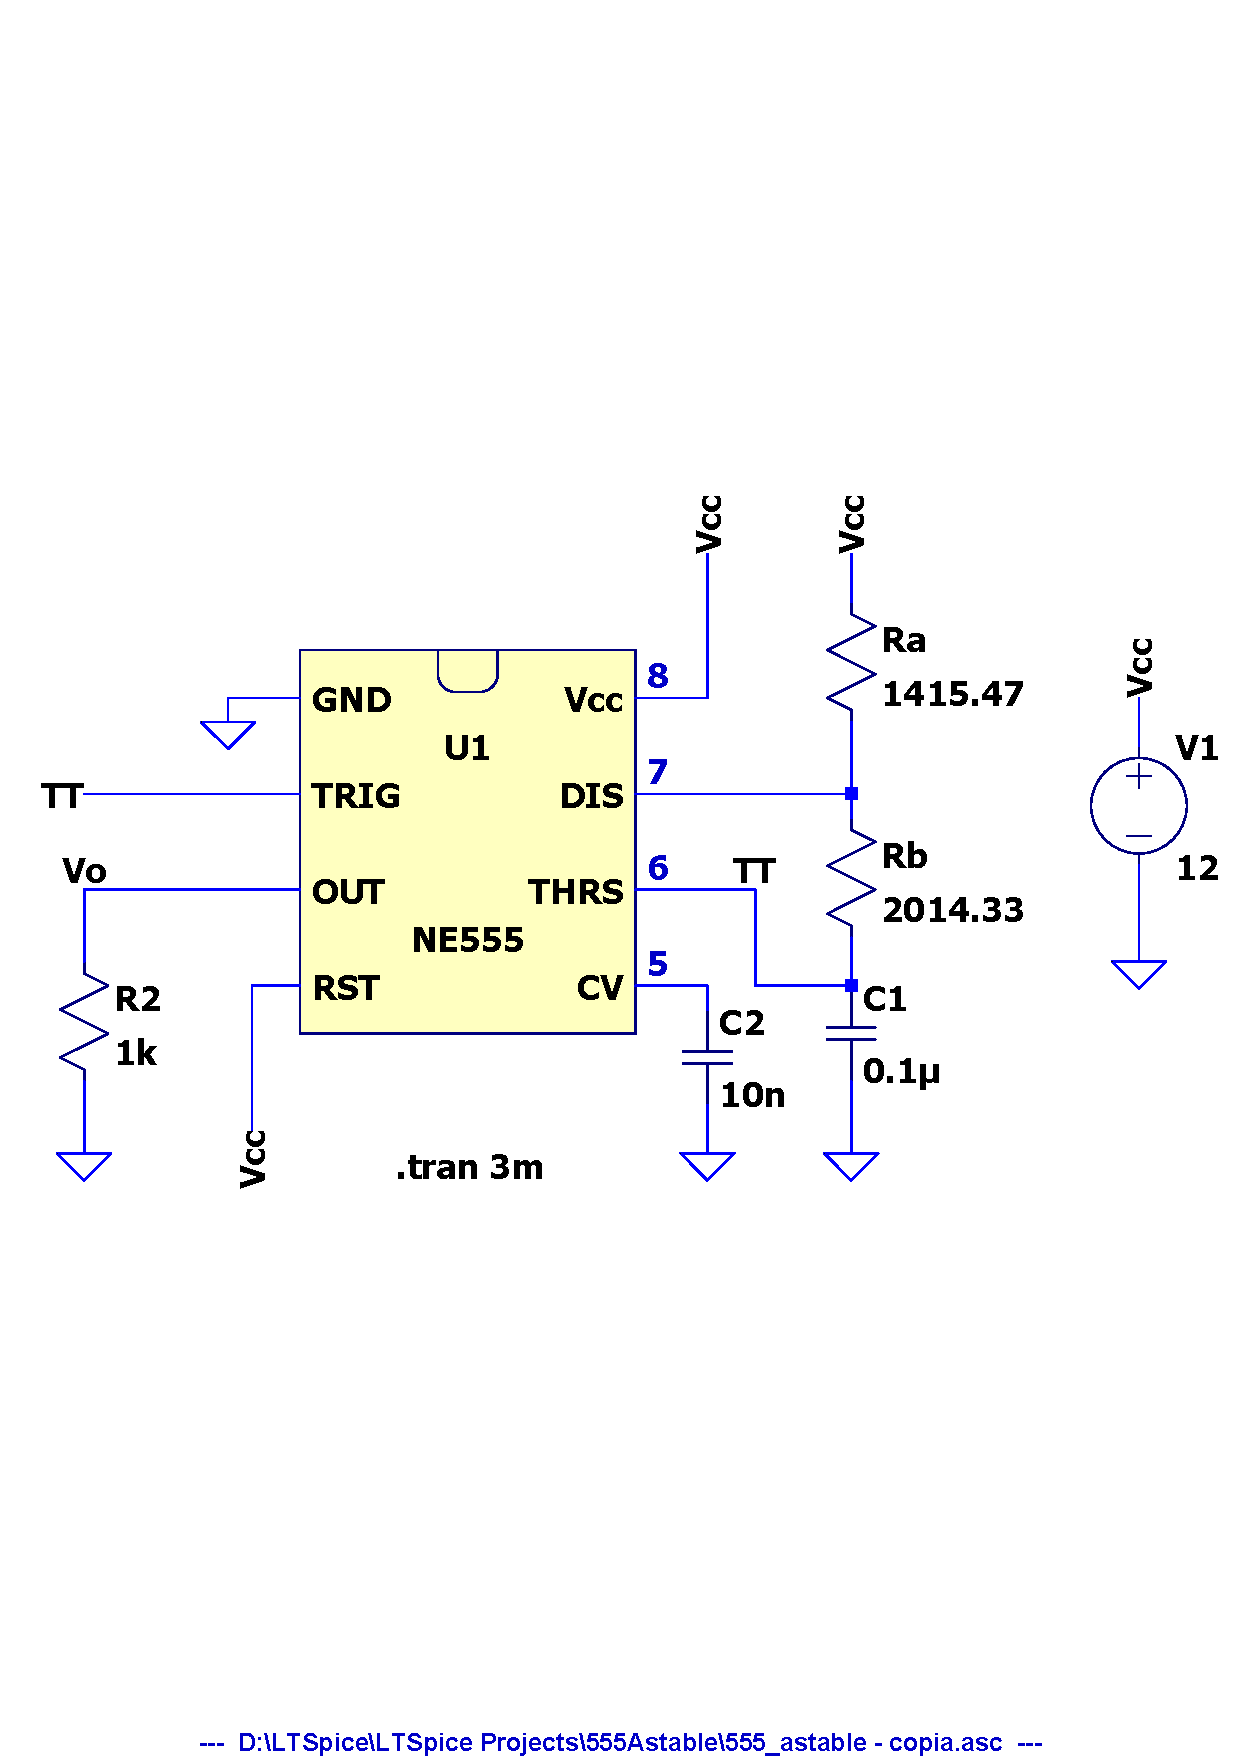
\includegraphics[clip, trim=1cm 8cm 0cm 7cm, width=0.9\textwidth]{Draft5}
\end{figure}

En la siguiente gráfica podemos observar la forma de onda de salida así como tres diferentes corrdenadas [t(ms), V(Volt)] con el cual podemos determinar el periodo, el tiempo de carga, el tiempo de descarga y el duty cycle de la señal, de las coordenadas dadas en la imagen, sólo nos interesa el eje horizontal o el tiempo para hacer los cálculos antes mencionados, por lo que ignoramos el valor de voltaje en cada caso.

Dados los siguientes puntos:

\begin{align}
	p_1 = (\qty{1.7421842}{\milli \second}) \nonumber \\
	p_2 = (\qty{1.9798715}{\milli \second}) \nonumber \\ 
	p_3 = (\qty{2.1199143}{\milli \second}) \nonumber
\end{align}

El tiempo de carga estaría dado por:

\begin{align}
	t_c = p_2 - p_1 = \qty{1.9798715}{\milli \second} - \qty{1.7421842}{\milli \second} = \qty{237.6873}{\micro \second} \nonumber \nonumber
\end{align}

El tiempo de descarga estaría dado por:
\begin{align}
	t_d = p_3 - p_2 = \qty{2.1199143}{\milli \second} - \qty{1.9798715}{\milli \second} = \qty{140.0428}{\micro \second} \nonumber \nonumber
\end{align}

El periodo total estaría dado por

\begin{align}
	T = t_c + t_d = \qty{237.6873}{\micro \second} + \qty{140.0428}{\micro \second} = \qty{377.7301}{\micro \second} \nonumber
\end{align}

Por tanto, la frecuencia es 
\begin{align}
	f = \frac{1}{T} = \frac{1}{\qty{237.6873}{\micro \second}} = \qty{ 2647.39294}{\hertz} \nonumber
\end{align}

Por último, el ciclo de trabajo está dado por:
\begin{align}
	D = \frac{t_c}{T} = \frac{\qty{237.6873}{\micro \second}}{\qty{377.7301}{\micro \second}} = 62.92\% \nonumber
\end{align}


\begin{figure}[H]
	\centering
	% trim=left botm right top
	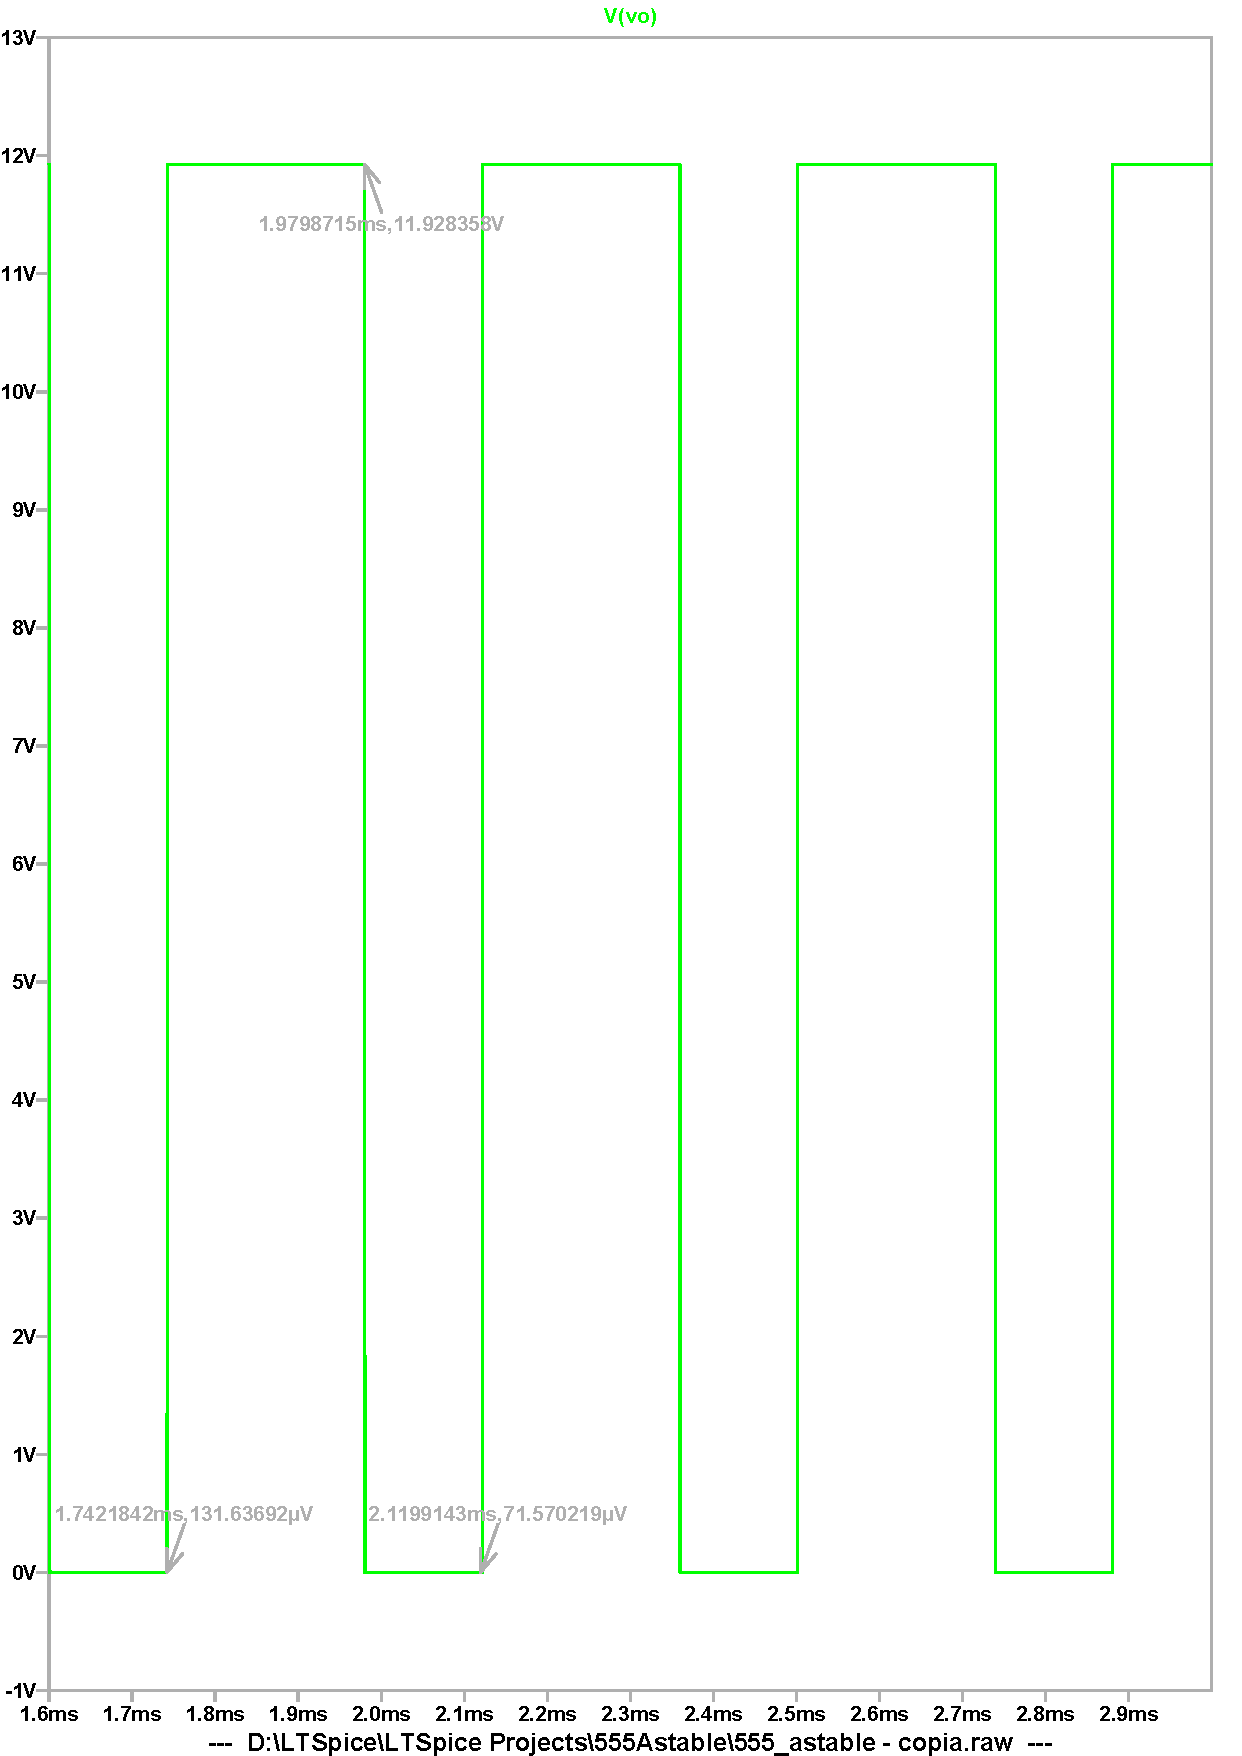
\includegraphics[clip, trim=0cm 0.5cm 0cm 0cm, width=0.9\textwidth]{Draft6}
\end{figure}

\newpage

\subsection*{Ejemplo 2}
Diseñe un multivibrador astable para que oscile a una frecuencia de 5-30 Hz. Escoja un valor de $C = \qty{0.1}{\mu \farad}$

Sea

\begin{align}
	T_1 &= \frac{1}{f_1} = \frac{1}{\qty{5}{\hertz}} = \qty{0.2}{\second} = \qty{200}{\milli \second} \nonumber \\
	T_2 &= \frac{1}{f_2} = \frac{1}{\qty{30}{\hertz}} = \qty{0.03333}{\second} = \qty{33.33}{\milli \second} \nonumber
\end{align}

Por conveniencia de diseño, el tiempo de carga será 2\% mayor que el tiempo de descarga (ya que el tiempo de carga y descarga no pñueden ser iguales), así, para el periodo $T_1$ el tiempo de carga será de

\begin{align}
	t_{c_1} = \frac{T_1}{2} + 2\% = \frac{T_1}{2} + \frac{2}{100}\frac{T_1}{2} = \qty{0.102}{\second}
\end{align}

El tiempo de descarga está dado por

\begin{align}
	t_{d_1} = T_1 - t_{c_1} = \qty{0.2}{\second} - \qty{0.102}{\second} = \qty{0.098}{\second} \nonumber
\end{align} 

Utilizamos la ecuación (44) para encontrar el valor de $R_B$

\begin{align}
	R_{B_{max}} = \frac{t_{d_1}}{C_1 \ln(2)} = \qty{1.4138}{\mega \ohm} \nonumber
\end{align}

De le ecuación (45), la resistencia $R_A$ tendrá un valor de

\begin{align}
	R_A = \frac{t_{c_1}}{C_1 \ln(2)} - R_B = \qty{57.75}{\kilo \ohm}\nonumber
\end{align}

Para el periodo $T_2$ el tiempo de carga está dado por
\begin{align}
	t_{c_2} = \frac{T_2}{2} + 2\% = \frac{T_2}{2} + \frac{2}{100}\frac{T_2}{2}  = \qty{0.017}{\second} \nonumber
\end{align}

De la ecuación (45) podemos despejar el valor de $R_B$ para obtener el valor de $R_{B_{min}}$
\begin{align}
	R_{B_{min}} = \frac{t_{c_2}}{C_1 \ln(2)} - R_A = \qty{187.51}{\kilo \ohm} \nonumber
\end{align}

\begin{figure}[H]
	\centering
	% trim=left botm right top
	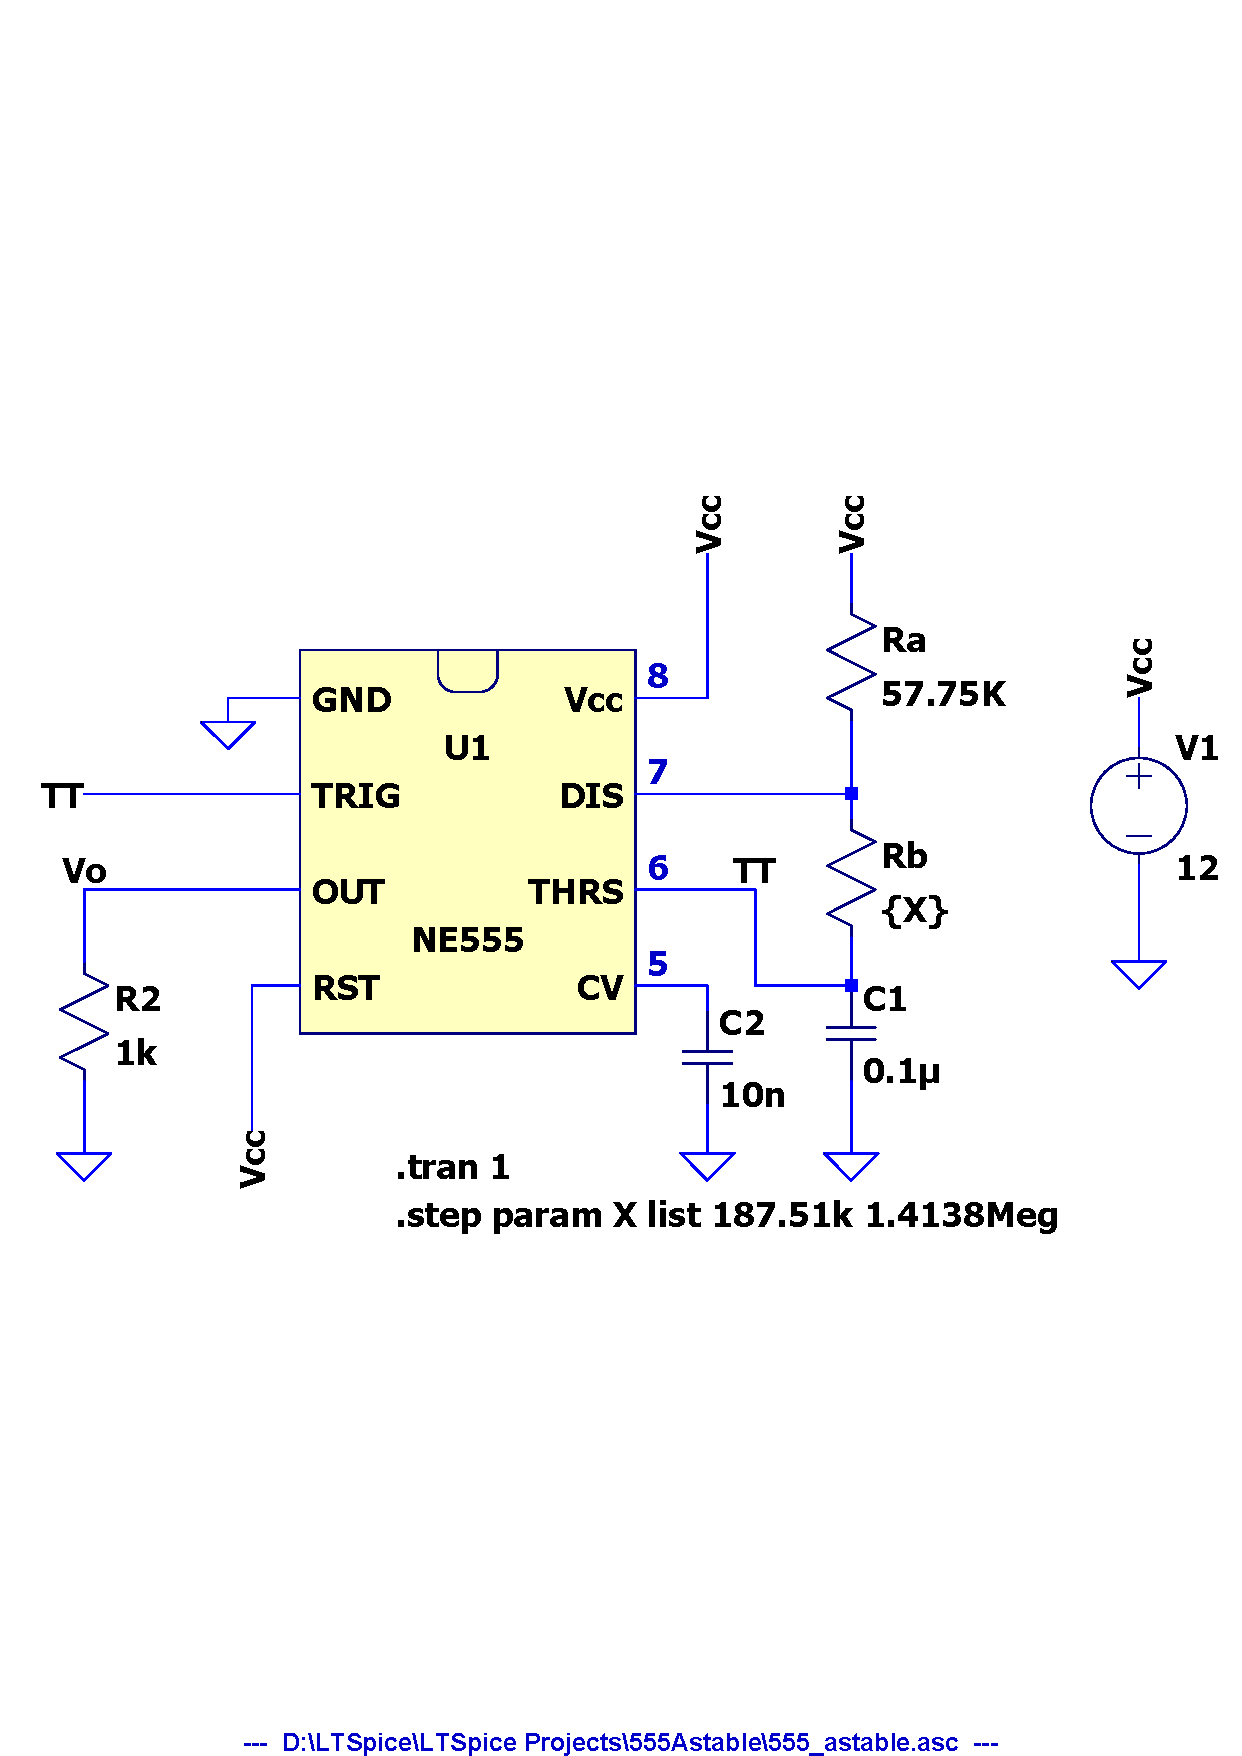
\includegraphics[clip, trim=1cm 8cm 0cm 7cm, width=0.9\textwidth]{Draft4}
\end{figure}

\begin{figure}[H]
	\centering
	% trim=left botm right top
	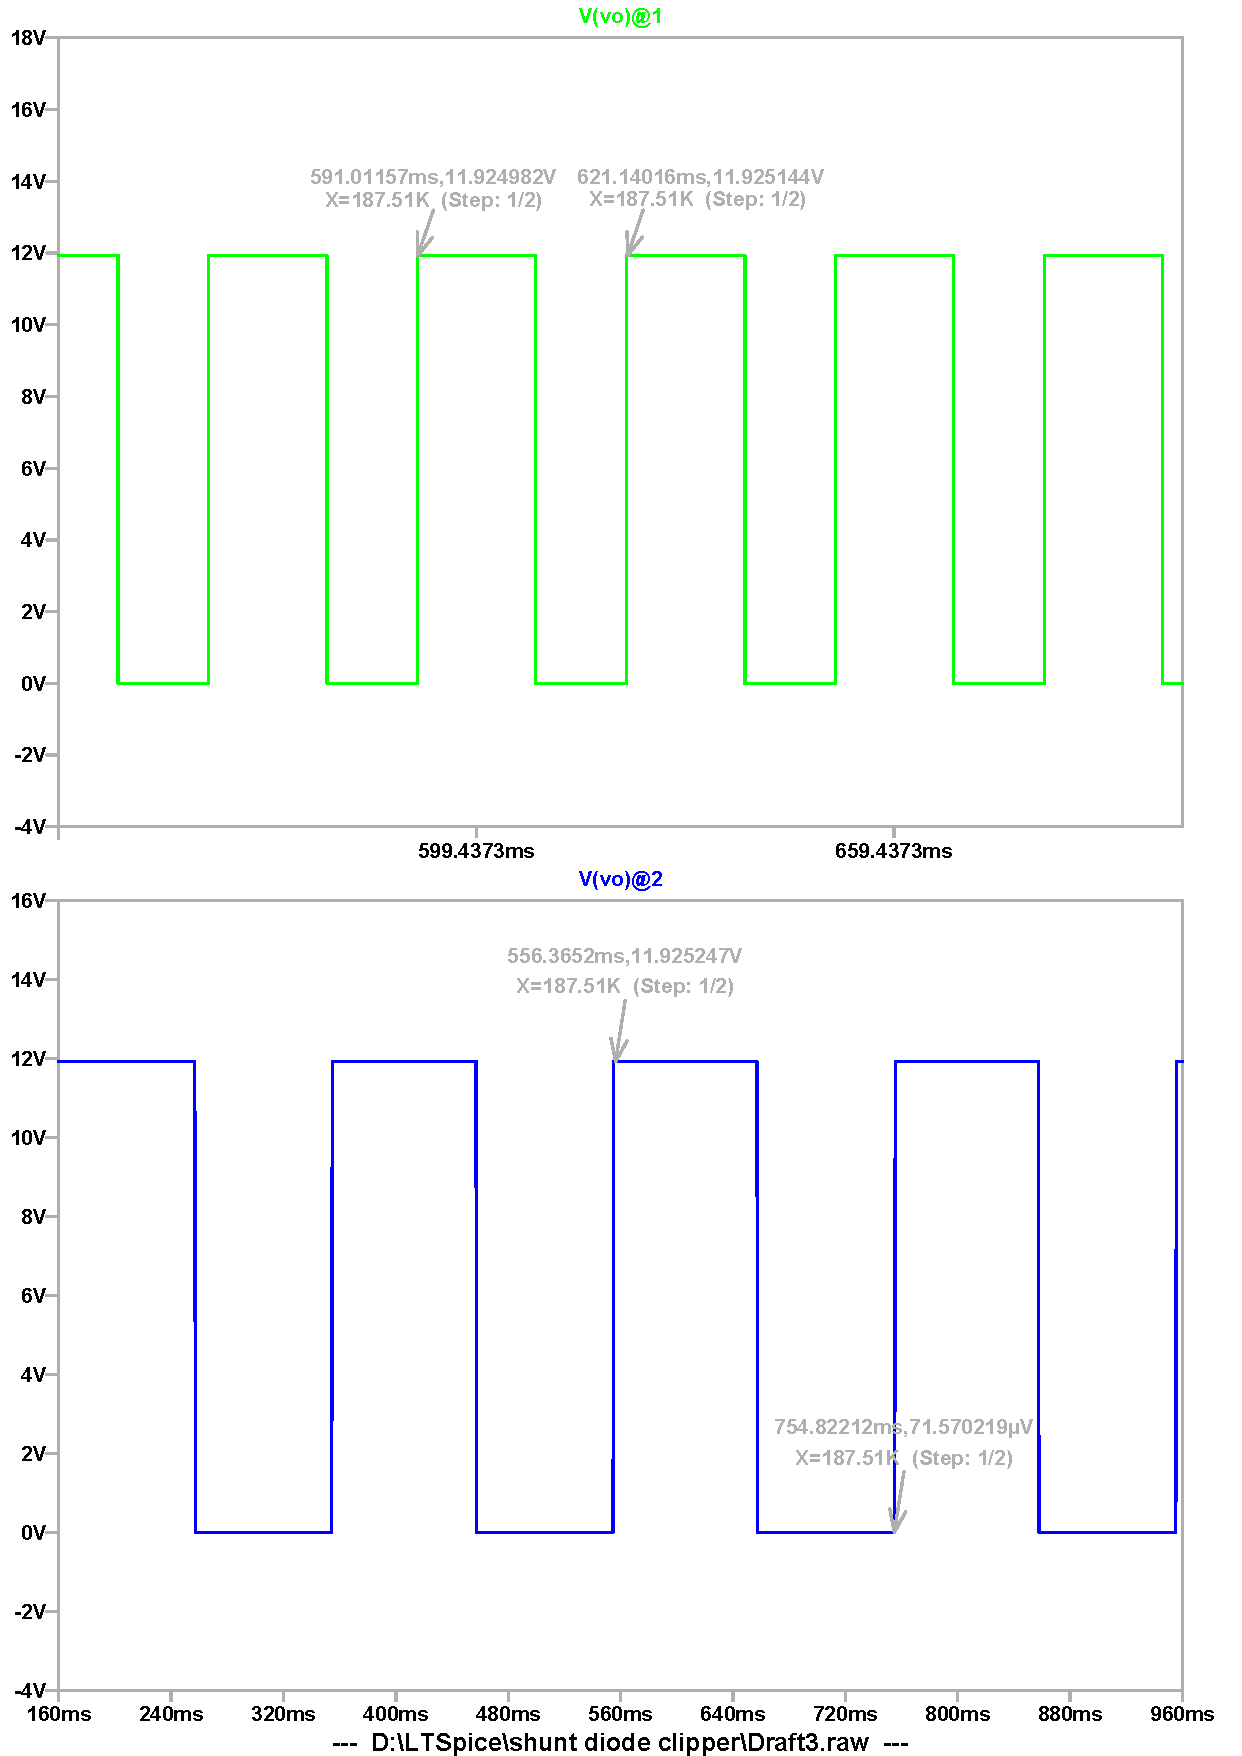
\includegraphics[clip, trim=0cm 0.5cm 0cm 0.1cm, width=\textwidth]{Draft3}
\end{figure}

\newpage

Prestemos atención en $R_B$, éste tiene un rango de valores, a saber, un valor mínimo de $\qty{187.51}{\kilo \ohm}$ y un valor máximo de $\qty{1.4138}{\mega \ohm}$. ¿Cómo podemos obtener ese rango de valores con resistencias y/o potenciómetros?, para esto, nos valemos de la siguiente configuración:

\begin{figure}[H]
	\centering	
	\begin{tikzpicture}[scale=0.8]
		\ctikzset{bipoles/thickness=4}
		\ctikzset{monopoles/vcc/arrow={Stealth[width=6pt,length=9pt]}}
		\ctikzset{monopoles/vee/arrow={Stealth[width=6pt,length=9pt]}}
		\draw (0,0) node[left]{$A$} to[R, l=$R_1$, o-*] ++(4,0) coordinate (p1) to[potentiometer, name=P, -*] node[left=10mm, below=2mm]{$R_p$} ++(4,0) to[short, -o] ++(2,0) node[right]{$B$};
		\draw(P.wiper) to[short] ++(0,1) coordinate (p2) to[short] (p2 -| p1) to[short] (p1);
		\draw (p1) to[short] ++(0,-3) to[R, l=$R_2$] ++(4,0) to[short] ++(0,3);
	\end{tikzpicture}
	\caption{}	
	\label{fig:figura16}
\end{figure}

Es claro ver que la resistencia entre los puntos $A,B$ está dada por

\begin{align}
	R_{AB} = R_1 + R_P \parallel R_2 = R_1 + \frac{R_2R_P}{R_2 + R_P}
\end{align}

Cuando la perilla del potenciómetro esté posicionada en su extremo inferior, la resistencia en $R_P$ será de $\qty{0}{\ohm}$ (idealmentw) por lo que $R_2$ estará cortocircuitada, haciendo que la resistencia entre los puntos $A,B$ sea de:


\begin{align}
	R_{AB} |_{\;R_P=0} = R_1 = R_{min}
\end{align}


Es decir, cuando la resistencia del potenciómetro esté a $\qty{0}{\ohm}$, la mínima resistencia que podemos obtener entre las terminales $A,B$ del circuito de la figura 16 es de $R_1$. \\

Es decir, recordemos que del circuito que diseñamos, $R_{B_{min}} = \qty{187.51}{\kilo \ohm}$ y $R_{B_{max}} = \qty{1.4138}{\mega \ohm}$. Si hacemos que $R_1$ sea igual a $R_{B_{min}}$ ($R_1 = R_{B_{min}}$) habremos resuelto la primera parte, ¿pero como logramos obtener el valor de resistencia máximo? o mejor dicho, ¿qué valor de $R_P$ o $R_2$ debo colcoar para lograr obtener el valor de resistencia máximo? \\

Para esto, es conveniente tener en cuenta que cuando se tienen dos resistencias en paralelo, el valor resultante de esas dos resistencias será menor que el valor de la resistencia más pequeña colocada en paralelo. Ahora, ¿qué pasa si uno coloca un valor de potenciómetro que es menor al valor máximo que uno quiere llegar? Volvemos al mismo ejemplo, mi meta es llegar a un valor máximo de resistencia de $\qty{1.4138}{\mega \ohm}$, ¿qué pasa si yo coloco un potenciómetro de $\qty{1}{\mega \ohm}$ por ejemplo? Antes de contestar esa última pregunta, hagamos otro supuesto. Supongamos que en el mejor de los casos, el valor de $R_2$ es lo sufucientemente alto ($R_2 \rightarrow$ $\infty$), por lo que el valor equivalente de $R_P$ y $R_2$ sería de $R_{eq}(R_P, R_2)|_{R_2 \rightarrow \infty} = R_P \parallel R_2 = R_P$. Cuando el potenciómetro esté en su valor máximo, la máxima resistencia que podríamos tener entre los puntos $A,B$ sería de

\begin{align}
	R_{AB}|_{R_2 \rightarrow \infty} = R_1 + R_P
\end{align}

Si sumamos los valores de $R_1$ y $R_P$ obtendríamos un valor de $R_{AB} = \qty{1.18751}{\mega \ohm}$ el cual está algo lejos de nuestra meta de $\qty{1.4138}{\mega \ohm}$. Supongamos que nuestro $R_{B_{max}}$ hubiese sido de $\qty{1.1}{\mega \ohm}$ en lugar de los $\qty{1.4138}{\mega \ohm}$, ahora en este caso, nos habríamos pasado. Con esto, queda claro, que el valor a escoger de $R_P$ siempre debe ser mayor que la resistencia máxima que deseamos, es decir:

\begin{align}
	R_P > R_{max}
\end{align}

Ahora, conociendo el valor de $R_1$ que será siempre nuestra resistencia mínima, y teniendo una idea clara de que $R_P$ debe ser siempre mayor que la resistencia máxima, podemos despejar sin problemas $R_2$ de la ecuación (48) para obtener:

\begin{align}
	R_{AB} = R_1 + \frac{R_2R_P}{R_2 + R_P} \nonumber \\
	R_{AB} - R_1 = \frac{R_2R_P}{R_2 + R_P} \nonumber \\
	(R_2 + R_P)(R_{AB} - R_1) = R_2R_P \nonumber \\
	R_2R_{AB} - R_2R_1 + R_PR_{AB} - R_PR_1 = R_2R_P \nonumber \\
	R_2R_{AB} - R_2R_1 - R_2R_P = R_PR_1 - R_PR_{AB} \nonumber \\
	R_2 (R_{AB} - R_1 - R_P) = R_P(R_1 -R_{AB}) \nonumber
\end{align}

Por lo tanto:

\begin{align}
	R_2 = \frac{R_P(R_1 -R_{AB})}{R_{AB} - R_1 - R_P} = \frac{R_P(R_{AB} - R_1)}{  R_1 + R_P - R_{AB}}
\end{align}

Así, si $R_1 = \qty{187.51}{\kilo \ohm}$, si seleccionamos un potenciómetro $R_P = \qty{2}{\mega \ohm}$ y queremos que nuestro $R_{ABmax}$ sea de \qty{1.4138}{\mega \ohm}, entonces el valor de $R_2$ deberá ser de

\begin{align}
	R_2 = \frac{(\qty{2}{\mega \ohm})( \qty{1.4138}{\mega \ohm} - \qty{187.51}{\kilo \ohm})}{\qty{187.51}{\kilo \ohm} + \qty{2}{\mega \ohm} - \qty{1.4138}{\mega \ohm}} \approx \qty{3.17}{\mega \ohm}
\end{align}

\begin{figure}[H]
	\centering	
	\begin{tikzpicture}[scale=0.7, transform shape]
		\ctikzset{muxdemux/inner label font=\small}
		\ctikzset{muxdemux/outer label font={\small\color{blue}}}
		\tikzset{ic555/.style={muxdemux,
				muxdemux def={Lh=10, NL=7, Rh=10, NR=1, NB=2, w=6, NT=2}, %Lh = Left height, Rh = Right Heigh, w = width, NL = number of pin on the left, NR, number of pín on the right, NB = number of pins on the bottom 
				muxdemux label={L2=Discharge, L5=Trigger, L6=Threshold, R1=Out,
					T1={\ctikztextnot{RST}}, T2=VCC,  B1=GND, B2=Control, 
					LU2=7, LU5=6, LU6=2, TL1=8, TL2=4, RU1=3, BL1=1, BL2=5},
				external pins width=0.4,
				draw only left pins={2,5,6},
				circuitikz/muxdemuxes/fill=blue!10}
		}
		\node [ic555, font=\small\ttfamily,align=center](A) at (0,0) {LM555};
		\draw (A.lpin 2) to[short] ++(-1,0) coordinate (p1);
		\draw (A.tpin 2) to[short] ++(0,1) coordinate (t2); %top pin2
		\draw (p1) to[R, l=$R_1$] (p1 |- t2) coordinate (r1) to [short] (t2);
		\draw (A.tpin 1) to[short, -*] ++(0,1) to[short] ++(0,0.2) node[vcc](VCC){$+V_{CC}$};
		\draw (A.lpin 5) to[short] ++(-1,0) coordinate (p6);
		\draw (p1) to[R, l_=$R_{b_{min}}$, *-*] ++(-4,0) coordinate (c1) to[potentiometer, name=P] node[left=5mm, above=7mm]{$R_P$} (c1 |- p6) coordinate (c3) to[short, -*] (p6);
		\draw (c1) to[short] ++(-2,0) coordinate (c2) to[R, l=$R_x$] (c2 |- p6) to[short, -*] (c3);
		\draw (P.wiper) to[short] ++(0.4,0) to[short, -*] ++(0,1.2);
		\draw (A.lpin 6) to[short, -*] ++(-1,0) coordinate (p2);
		\draw (p2) to[short] (p6);
		\draw (p2) to[cC, l_=$C_1$] ++(0,-3) coordinate (c1);
		\draw (A.bpin 1) to[short, -*] (c1 -| A.bpin 1) coordinate (pgnd);
		\draw (A.bpin 2) to[cC, l=$C_2$] (c1 -| A.bpin 2) --(pgnd);
		\draw (c1) to[short] (pgnd) node[ground]{};
		\draw (A.rpin 1) to[short, -o] ++(0.5,0);
	\end{tikzpicture}
	\caption{Multivibrador astable ajustado para un rango de frecuencias}	
	\label{fig:figura17}
\end{figure}

\end{document}